\documentclass[conference]{IEEEtran}

%\usepackage[numbers, sort, compress]{natbib}
\usepackage{graphicx}
\usepackage{amsmath}
\usepackage{amssymb}
\usepackage{color}
\usepackage{ifpdf}
%\usepackage{mdwlist}

%\usepackage{dcolumn}
\usepackage{float}
\usepackage[utf8]{inputenc}
\usepackage{multirow}
\usepackage{rotating}
\usepackage{subfigure}

\usepackage{moresize}
%\usepackage{setspace}

%\usepackage[numbers, sort, compress]{natbib}
%\usepackage{latex8}
%\usepackage{float}
%\usepackage{times}    
\usepackage{url}
\usepackage{booktabs}
\usepackage{listings}   
\usepackage{paralist}    
\usepackage{wrapfig}    
%\usepackage[footnotesize,it]{caption}
\usepackage{multirow}
\usepackage{ifpdf}
%\usepackage{srcltx}
%\usepackage{subfigure}
\usepackage{xspace}
\usepackage{keyval}  
\usepackage{color}

\definecolor{listinggray}{gray}{0.95}
\definecolor{darkgray}{gray}{0.7}
\definecolor{commentgreen}{rgb}{0, 0.4, 0}
\definecolor{darkblue}{rgb}{0, 0, 0.4}
\definecolor{middleblue}{rgb}{0, 0, 0.7}
\definecolor{darkred}{rgb}{0.4, 0, 0}
\definecolor{brown}{rgb}{0.5, 0.5, 0}
\definecolor{dkgreen}{rgb}{0,0.5,0}
\definecolor{orange}{rgb}{1,.5,0}
\definecolor{dandelion}{cmyk}{0,0.29,0.84,0}

\usepackage[normalem]{ulem}
\makeatletter
\def\cyanuwave{\bgroup \markoverwith{\lower3.5\p@\hbox{\sixly \textcolor{cyan}{\char58}}}\ULon}
\def\reduwave{\bgroup \markoverwith{\lower3.5\p@\hbox{\sixly \textcolor{red}{\char58}}}\ULon}
\def\blueuwave{\bgroup \markoverwith{\lower3.5\p@\hbox{\sixly \textcolor{blue}{\char58}}}\ULon}
\font\sixly=lasy6 % does not re-load if already loaded, so no memory problem.
\makeatother


%\usepackage{xcolor}
\newif\ifdraft
\drafttrue
\ifdraft
 \newcommand{\N}[1]{\textbf{NOTE: #1}\xspace}
 \newcommand{\jhanote}[1]{ {\textcolor{red} { ***SJ: #1 }}}
 \newcommand{\katznote}[1]{ {\textcolor{blue} { ***DSK: #1 }}}
 \newcommand{\mtnote}[1]{ {\textcolor{orange} { ***MT: #1 }}}
 \newcommand{\jonnote}[1]{ {\textcolor{dkgreen} { ***JW: #1 }}}
  \newcommand{\aanote}[1]{ {\textcolor{dkgreen} { ***AA: #1 }}}
 \newcommand{\note}[1]{ {\textcolor{brown} { *** #1 }}}
\else
 \newcommand{\N}[1]{}
 \newcommand{\jhanote}[1]{}
 \newcommand{\katznote}[1]{}
 \newcommand{\mtnote}[1]{}
 \newcommand{\jonnote}[1]{}
 \newcommand{\note}[1]{}
\fi

\newif\ifdraft
%\drafttrue
\ifdraft
\newcommand{\terminology}[1]{ {\textcolor{red} {(Terminology used: \textbf{#1}) }}}
\newcommand{\owave}[1]{ {\cyanuwave{#1}}}
\newcommand{\jwave}[1]{ {\reduwave{#1}}}
\newcommand{\alwave}[1]{ {\blueuwave{#1}}}
\newcommand{\alnote}[1]{ {\textcolor{blue} { ***andreL: #1 }}}
\newcommand{\amnote}[1]{ {\textcolor{blue} { ***andreM: #1 }}}
\newcommand{\smnote}[1]{ {\textcolor{brown} { ***sharath: #1 }}}
\newcommand{\pmnote}[1]{ {\textcolor{brown} { ***Pradeep: #1 }}}
\newcommand{\msnote}[1]{ {\textcolor{cyan} { ***mark: #1 }}}
\newcommand{\mrnote}[1]{ {\textcolor{purple} { ***melissa: #1 }}}
%\newcommand{\mtnote}[1]{ {\textcolor{orange} { ***matteo: #1 }}}
\else
\newcommand{\onote}[1]{}
\newcommand{\terminology}[1]{}
\newcommand{\owave}[1]{#1}
\newcommand{\jwave}[1]{#1}
\newcommand{\alnote}[1]{}
\newcommand{\amnote}[1]{}
\newcommand{\athotanote}[1]{}
\newcommand{\smnote}[1]{}
\newcommand{\pmnote}[1]{}
\newcommand{\msnote}[1]{}
\newcommand{\mrnote}[1]{}
\newcommand{\aznote}[1]{}
%\newcommand{\mtnote}[1]{}
\fi

\newcommand{\cloud}{cloud\xspace}
\newcommand{\clouds}{clouds\xspace}
\newcommand{\pilot}{Pilot\xspace}
\newcommand{\pilots}{Pilots\xspace}
\newcommand{\pilotjob}{Pilot-Job\xspace}
\newcommand{\pilotjobs}{Pilot-Jobs\xspace}
\newcommand{\pilotcompute}{Pilot-Compute\xspace}
\newcommand{\pilotcomputedescription}{Pilot-Compute Description\xspace}
\newcommand{\pilotdescription}{Pilot-Description\xspace}
\newcommand{\pilotcomputes}{Pilot-Computes\xspace}
\newcommand{\pilotdata}{Pilot-Data\xspace}
\newcommand{\pilotdatadescription}{Pilot-Data Description\xspace}
\newcommand{\pilotdataservice}{Pilot-Data Service\xspace}
\newcommand{\pilotcomputeservice}{Pilot-Compute Service\xspace}
\newcommand{\computedataservice}{Compute-Data Service\xspace}
\newcommand{\computeunitdescription}{Compute-Unit Description\xspace}
\newcommand{\dataunitdescription}{Data-Unit Description\xspace}
\newcommand{\pilotmapreduce}{PilotMapReduce\xspace}
\newcommand{\mrmg}{MR-Manager\xspace}
\newcommand{\pstar}{P*\xspace}
\newcommand{\pd}{PD\xspace}
\newcommand{\pc}{PC\xspace}
\newcommand{\pcs}{PCs\xspace}
\newcommand{\pj}{PJ\xspace}
\newcommand{\pjs}{PJs\xspace}
\newcommand{\pds}{Pilot Data Service\xspace}
\newcommand{\computeunit}{Compute-Unit\xspace}
\newcommand{\computeunits}{Compute-Units\xspace}
\newcommand{\dataunit}{Data-Unit\xspace}
\newcommand{\dataunits}{Data-Units\xspace}
\newcommand{\du}{DU\xspace}
\newcommand{\dus}{DUs\xspace}
\newcommand{\dud}{DUD\xspace}
\newcommand{\cu}{CU\xspace}
\newcommand{\cus}{CUs\xspace}
\newcommand{\cud}{CUD\xspace}
\newcommand{\su}{SU\xspace}
\newcommand{\sus}{SUs\xspace}
\newcommand{\schedulableunit}{Schedulable Unit\xspace}
\newcommand{\schedulableunits}{Schedulable Units\xspace}
\newcommand{\cc}{c\&c\xspace}
\newcommand{\CC}{C\&C\xspace}
\newcommand{\up}{\vspace*{-1em}}
\newcommand{\upp}{\vspace*{-0.5em}}
\newcommand{\numrep}{8 }
\newcommand{\samplenum}{4 }
\newcommand{\tmax}{$T_{max}$ }
\newcommand{\tc}{$T_{C}$ }
\newcommand{\tcnsp}{$T_{C}$}
\newcommand{\bj}{BigJob\xspace}
\newcommand{\irods}{iRODS\xspace}

\newcommand{\I}[1]{\textit{#1}\xspace}
\newcommand{\B}[1]{\textbf{#1}\xspace}
\newcommand{\T}[1]{\texttt{#1}\xspace}
\newcommand{\C}[1]{\textsc{#1}\xspace}

\newcommand{\mr}[1]{\multirow{2}{*}{#1}}%
\newcommand{\mc}[2]{\multicolumn{#1}{l}{#2}}

\lstdefinestyle{myListing}{
  frame=single,   
  backgroundcolor=\color{listinggray},  
  %float=t,
  language=C,       
  basicstyle=\ttfamily \footnotesize,
  breakautoindent=true,
  breaklines=true
  tabsize=2,
  captionpos=b,  
  aboveskip=0em,
  belowskip=-2em,
  %numbers=left, 
  %numberstyle=\tiny
}      

\lstdefinestyle{myPythonListing}{
  frame=single,   
  backgroundcolor=\color{listinggray},  
  %float=t,
  language=Python,       
  basicstyle=\ttfamily \scriptsize,
  breakautoindent=true,
  breaklines=true
  tabsize=2,
  captionpos=b,  
  %numbers=left, 
  %numberstyle=\tiny
}



%  \setlength{\parskip}{0.05ex} % 1ex plus 0.5ex minus 0.2ex}
%  \setlength{\parsep}{0pt}
%  %\setlength{\headsep}{0pt}
%  \setlength{\topskip}{0pt}
%  \setlength{\topmargin}{0pt}
%  %\setlength{\topsep}{0pt}
%  \setlength{\partopsep}{0pt}

% This is now the recommended way for checking for PDFLaTeX:


\ifpdf
\DeclareGraphicsExtensions{.pdf, .jpg, .tif}
\else
\DeclareGraphicsExtensions{.ps,  .eps, .jpg}
\fi

\tolerance=1000
\hyphenpenalty=10


% -----------------------------------------------------------------------------
% BEGIN DOCUMENT
% -----------------------------------------------------------------------------
\begin{document}

\title{Converging High-Throughput and High-Performance Computing: A Case Study}

\author{
    \IEEEauthorblockN{
        Alessio Angius\IEEEauthorrefmark{1}\IEEEauthorrefmark{2},
        Danila Oleynik\IEEEauthorrefmark{1}\IEEEauthorrefmark{5},
        Sergey Panitkin\IEEEauthorrefmark{1}\IEEEauthorrefmark{4},
        Matteo Turilli\IEEEauthorrefmark{1}\IEEEauthorrefmark{2},\\
        Kaushik De\IEEEauthorrefmark{5},
        Alexei Klimentov\IEEEauthorrefmark{4},
        Sarp H. Oral\IEEEauthorrefmark{6},
        Jack C. Wells\IEEEauthorrefmark{6} and
        Shantenu Jha\IEEEauthorrefmark{2}
    }
    \IEEEauthorblockA{
        \IEEEauthorrefmark{1}First authors, alphabetical order
    }
    \IEEEauthorblockA{
        \IEEEauthorrefmark{2}Department of Electric and Computer Engineering, Rutgers University, NJ, USA
    }
    \IEEEauthorblockA{
        \IEEEauthorrefmark{4}Physics Department, Brookhaven National Laboratory, NY, USA
    }
    \IEEEauthorblockA{
        \IEEEauthorrefmark{5}Physics Department, University of Texas Arlington, TX, USA
    }
    \IEEEauthorblockA{
        \IEEEauthorrefmark{6}Oak Ridge Leadership Computing Facility, Oak Ridge National Laboratory, TN, USA
    }
}

\maketitle

% ----------------------------------------------------------------------------
% ABSTRACT
% ----------------------------------------------------------------------------
\begin{abstract}
The computing systems used by LHC experiments has historically consisted of
the federation of hundreds to thousands of distributed resources, ranging from
small to mid-size resource.  In spite of the impressive scale of the existing
distributed computing solutions, the federation of small to mid-size
resources will be insufficient to meet projected future demands.
This paper is a case study of how the ATLAS experiment has embraced Titan -- a
DOE leadership facility in conjunction with traditional distributed high-
throughput computing to reach sustained production scales of approximately 51M
core-hours a years. The three main contributions of this paper are:  (i) a
critical evaluation of design and operational considerations  to support the
sustained, scalable and production usage of Titan;  (ii) a preliminary
characterization of a next generation executor for PanDA to support new
workloads and  advanced execution modes; and (iii) early lessons for how
current and future experimental and observational systems can be integrated
with production supercomputers and other platforms in a general and extensible
manner.
\end{abstract}

\begin{IEEEkeywords}
Distributed Computing, Workload Management System.
\end{IEEEkeywords}

% ----------------------------------------------------------------------------
% I - INTRODUCTION
% ----------------------------------------------------------------------------
\section{Introduction}
\label{sec:intro}

The Large Hadron Collider (LHC) was created to explore the fundamental
properties of matter for the next decades. Multiple experiments at LHC have
collected and distributed hundreds of petabytes of data worldwide to hundreds of
computer centers. Thousands of physicists analyze petascale data volumes daily.
The detection of the Higgs Boson in 2013 speaks to the success of the detector
and experiment design, as well as the sophistication of computing systems
devised to analyze the data.

Historically, the computing systems used by LHC experiments consisted of the
federation of hundreds to thousands of distributed resources, %\textemdash{}
ranging in scale from small to mid-size resource~\cite{foster2003grid}. Although
the workloads to be executed are comprised of tasks that are independent of each
other, the management of the distribution of workloads across many heterogeneous
resources to ensure the effective utilization of resources and efficient
execution of workloads presents non-trivial challenges.

Many software solutions have been developed in response to these challenges.
CMS, one of the LHC experiments, devised a solution based around the
HTCondor~\cite{thain2005distributed} software ecosystem. The
ATLAS~\cite{Aad:2008} experiment, utilizes the Production and Distributed
Analysis (PanDA) workload management system~\cite{Maeno2011} (WMS) for
distributed data processing and analysis. The CMS and ATLAS experiments
represent arguably the largest production grade distributed computing solutions
and have symbolized the paradigm of {\it high-throughput computing}, i.e., the
effective execution of many independent tasks.

As the LHC prepares for Run 3 in $~\approx$ 2022 and the high-luminosity era
(Run 4), it is anticipated that the data volumes that will need analyzing will
increase by factors of 10-100 compared to the current phase (Run 2). Data will
be larger in volume but will also require more sophisticated computational
processing. In spite of the impressive scale of the ATLAS distributed computing
system, demand for computing systems will significantly outstrip current and projected supply.

There are multiple levels at which this problem needs to be addressed: the
utilization of emerging parallel architectures (e.g., platforms); algorithmic
and advances in analytical methods (e.g., use of Machine Learning); and the
ability to exploit different platforms (e.g., clouds and supercomputers).

This paper is a case study of how the ATLAS experiment has ``broken free'' of
the traditional computational approach of high-throughput computing on
distributed resources to embrace new platforms, in particular high-performance
computers. Specifically, we discuss the experience of integrating PanDA WMS with
a DOE leadership computing facility called Titan to reach sustained production
scales of approximately 51M core-hours a year. We also discusses the
investigation of a task execution runtime system on Titan, that is based on the
pilot-abstractions and which allows advanced execution modes of the ATLAS
workload as well as the enhanced support for heterogeneous workloads such as
molecular dynamics.

This state-of-practice paper provides three main contributions:  (i) a critical
evaluation of the many design and operational considerations that have been
taken to support the sustained, scalable and production usage of Titan for
historically high-throughput workloads; (ii) a preliminary characterization of a
next generation executor (NGE) for PanDA to support non-traditional
heterogeneous workloads and execution modes;  and (iii) early lessons and
guidance as the community looks forward to designing the next generation of
online analytical platforms~\cite{foap-url}, for how current and future
experimental and observational systems can be integrated with production
supercomputers in a general and extensible manner.

% ----------------------------------------------------------------------------
% II - PanDA OVERVIEW
% ----------------------------------------------------------------------------
\section{PanDA Overview}
\label{sec:panda_overview}

PanDA is a Workload Management System (WMS)~\cite{marco2009glite} designed to
support the execution of distributed workloads and workflows via
pilots~\cite{turilli2015comprehensive}. Pilot-capable WMS enable high throughput
of tasks execution via multi-level scheduling while supporting interoperability
across multiple sites. This is particularly relevant for LHC experiments, where
millions of tasks are executed across multiple sites every month, analyzing and
producing petabytes of data. The design of PanDA WMS started in 2005 to support
ATLAS. PanDA went into production for the LHC Run 1 on 2009, and was then
extended with new subsystems for Run 2 in 2015.


% -----------------------------------------------------------------------------
\subsection{Design}
\label{ssec:panda_design}

PanDA's application model assumes tasks grouped into workloads and workflows.
Tasks represent a set of operations performed on data sets stored in one or more
input files. Tasks are decomposed into jobs, where each job consists of the
task's operations performed on a partition of the task's data set. Since 2005, a
certain amount of parallelism has been progressively introduced for job
execution~\cite{crooks2012multi} but, so far, HEP applications have not required
a message passing interface (MPI).
% Jobs are supposed to be capable of setting up their own execution
% environment and have a minimal set of common dependences.

PanDA's usage model assumes multitenancy of resources and at least two types of
HEP users: individual researchers and groups executing so called `production'
workflows.
% Users can submit tasks and workflows to the PanDA WMS at any point in
% time, directly or via dedicated application frameworks.
PanDA's security model is based on separation between authentication,
authorization and accounting for both single users and group of users. Both
authentication and authorization are based on digital certificates and on the
virtual organization abstraction~\cite{foster2001anatomy}.

Currently, PanDA's execution model is based on four main abstractions: task,
job, queue, and pilot. Both tasks and jobs are assumed to have attributes and
states and to be queued into a global queue for execution. Prioritization and
binding of jobs are assumed to depend on the attributes of each job. Pilot is
used to indicate the abstraction of resource capabilities. Each job is thought
to be bound to one pilot and executed on the site where the pilot has been
instantiated.

In PanDA's data model, each datum refers to the recorded or simulated
measurement of a physical process. Data can be packaged into files or other
containers. As with jobs, data have both attributes and states, and some of the
attributes are shared between events and jobs. Raw, reconstruction, and
simulation data are assumed to be distributed across multiple storage facilities
and managed by the ATLAS Distributed Data Management
(DDM)~\cite{garonne2012atlas}. When necessary, datasets required by each job are
assumed to be replicated over the network, both for input and output data.

PanDA's design supports provenance and traceability for both jobs and data.
Attributes enable provenance by linking jobs and data items, providing
information like ownership or project affiliation. States enable traceability by
providing information about the stage of the execution in which each job or data
item is or has been.
% Some attributes are assumed to be immutable across execution and jobs and data
% items are assumed to be always in one and only one state.


% -----------------------------------------------------------------------------
\subsection{Implementation and Execution}
\label{ssec:panda_arch}

The implementation of PanDA WMS consists of several interconnected subsystems,
most of them built from off-the-shelf and Open Source components. Subsystems
communicate via dedicated API or HTTP messaging, and each subsystem is
implemented by one or more modules. Databases are used to store eventful
entities  like tasks, jobs and  input/output data, and to store information
about sites, resources, logs, and accounting.

Currently, PanDA's architecture has five main subsystems: PanDA
Server~\cite{maeno2011overview},
AutoPyFactory~\cite{caballero2012autopyfactory}, PanDA
Pilot~\cite{nilsson2011atlas}, JEDI~\cite{borodin2015scaling}, and PanDA
Monitoring~\cite{klimentov2011atlas}. Other subsystems are used by some of ATLAS
workflows (e.g., PanDA Event Service~\cite{calafiura2015atlas}), but we do not
discuss them as they are  not relevant to an understanding of how PanDA has been
ported to supercomputers. For a full list of subsystems see
Ref.~\cite{panda-wiki_url}. Fig.~\ref{fig:architecture} shows a diagrammatic
representation of PanDA main subsystems, highlighting the execution process of
tasks while omitting monitoring details to improve readability.

\begin{figure}
    \centering
    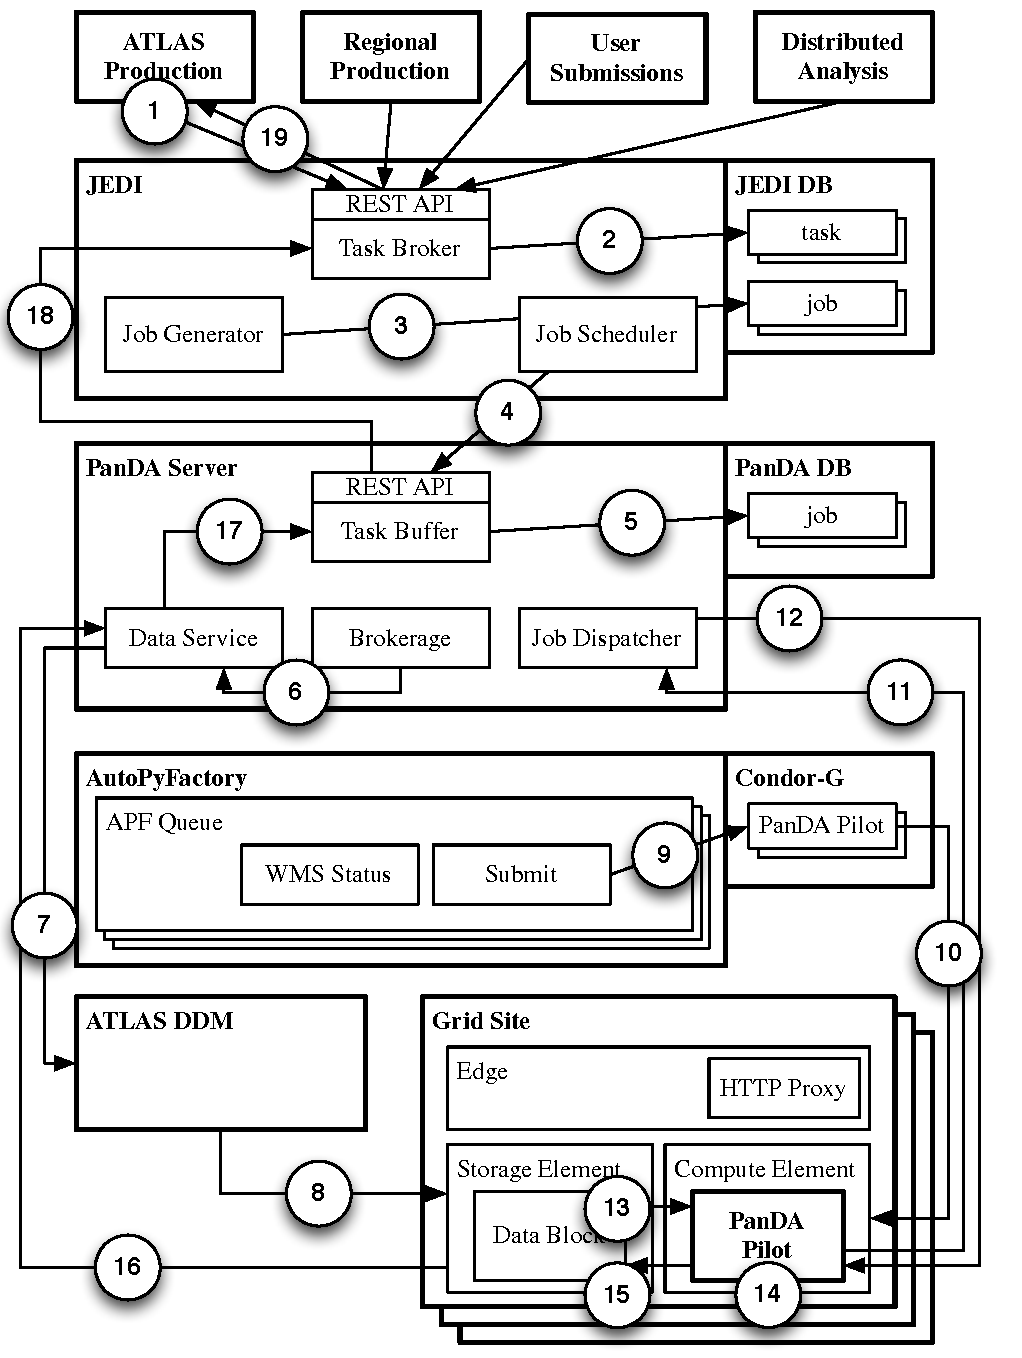
\includegraphics[width=\columnwidth]{panda_architecture.pdf}
    \caption{PanDA WMS architecture. Numbers indicates the JEDI-based execution
    process. Several subsystems, components, and architectural and
    communication details are abstracted to improve clarity.}
\label{fig:architecture}
\end{figure}

During LHC Run 1, PanDA required users to perform a static conversion between
tasks and jobs: tasks were described as a set of jobs and then submitted to the
PanDA Server. This introduced inefficiency both with usability and resource
utilization~\cite{borodin2015unified}. Ideally, users should conceive analyses
in terms of one or more, possibly related tasks, while the execution manager
(i.e., PanDA) should partition tasks into jobs, depending on execution
constraints. Further, the static partitioning of tasks into jobs does not take
into account the heterogeneity and dynamicity of the resources on which each job
will be executed, introducing inefficiencies.

Another problem of static job sizing is that PanDA instantiates pilots on sites
with different type of resources and different models of availability of those
resources. An optimal sizing of each job should take into account these
properties. For example, sites may offer cores with different speed, networking
with different amount of bandwidth, and resources could be guaranteed to be
available for a defined amount of time or could disappear at any point in time
as it happens with opportunistic models of resource provision.

JEDI was deployed for the LHC Run 2 to address these inefficiencies. Users
submit task descriptions to JEDI (Fig.~\ref{fig:architecture}:1) that stores
them into a queue implemented by a database (Fig.~\ref{fig:architecture}:2).
Tasks are partitioned into jobs of different size, depending on both static and
dynamic information about available resources (Fig.~\ref{fig:architecture}:3).
Jobs are bound to sites with resources that best match jobs' requirements, and
submitted to the PanDA Server for execution (Fig.~\ref{fig:architecture}:4).

Once submitted to the PanDA Server, jobs are stored by the Task Buffer component
into a global queue implemented as a database (Fig.~\ref{fig:architecture}:5).
When jobs are submitted directly to the PanDA Server, the Brokerage component is
used to bind jobs to available sites, depending on static information about the
resources available for each site. Jobs submitted by JEDI are already bound to
sites so no further brokerage is needed.

Once jobs are bound to sites, the Brokerage module communicates to the Data
Service module what data sets need to be made available on what site
(Fig.~\ref{fig:architecture}:6). The Data Service communicates these
requirements to the ATLAS DDM (Fig.~\ref{fig:architecture}:7) that, when needed,
replicates data sets on the required sites (Fig.~\ref{fig:architecture}:8).

Meanwhile, AutoPyFactory defines PanDA Pilots, submitting them to a Condor-G
agent (Fig.~\ref{fig:architecture}:9). Condor-G schedules these pilots wrapped
as jobs or VMs to the required sites (Fig.~\ref{fig:architecture}:10).

When a PanDA Pilot becomes available, it requests the Job Dispatcher module of
the PanDA Server for a job to execute (Fig.~\ref{fig:architecture}:11). The Job
Dispatcher interrogates the Task Buffer module for a job that is bound to the
site of that pilot and ready to be executed. Task Buffer checks the global queue
(i.e., the PanDA database) and, upon availability, returns a job to the Job
Dispatcher. The Job Dispatcher dispatches that job to the PanDA Pilot
(Fig.~\ref{fig:architecture}:12).

Upon receiving a job, a PanDA Pilot starts a monitoring process and forks a
subprocess for the execution of the job's payload. Input data are transferred
from the stage-in location (Fig.~\ref{fig:architecture}:13) and the job's
payload is executed (Fig.~\ref{fig:architecture}:14). Once completed, output is
transferred to the staging-out location (Fig.~\ref{fig:architecture}:15).

The Data Service module of the PanDA Server tracks and collects the output
generated by each job (Fig.~\ref{fig:architecture}:16), updating jobs'
attributes via the Task Buffer module (Fig.~\ref{fig:architecture}:17). When the
output of all the jobs of a task are retrieved, it is made available to the user
via PanDA Server. When a task is submitted to JEDI, task is instead marked as
done (Fig.~\ref{fig:architecture}:18) and the result of its execution is made
available to the user by JEDI (Fig.~\ref{fig:architecture}:19).


% ----------------------------------------------------------------------------
% III - DEPLOYING PANDA ON A LEADERSHIP-SCALE SYSTEM
% ----------------------------------------------------------------------------
%\section{Deploying PanDA on a Leadership-scale system}
\section{Deploying PanDA on Titan}
\label{sec:panda_titan}

The upcoming LHC Run 3 will require more resources than the Worldwide LHC
Computing Grid (WLCG) can provide. Currently, PanDA WMS uses more than 300,000
cores at over 100 Grid sites, with a peak performance of 0.3 petaFLOPS. This
capacity will be sufficient for the planned analysis and data processing, but it
will be insufficient for the Monte Carlo production workflow and any extra
activity. To alleviate these challenges, ATLAS is expanding the current
computing model to include additional resources such as the opportunistic use of
supercomputers.

Generally, supercomputers are designed to support parallel computation that
requires runtime communication. Jobs are executed across multiple cores, each
core calculating a small part of the problem and communicating with other cores
via MPI. Accordingly, supercomputers have large number of worker nodes,
connected through a high-speed, low-latency dedicated network. Each worker node
has multicore CPUs, usually augmented with Graphics Processing Units (GPUs) or
other specialized coprocessors.

PanDA WMS has been designed to support distributed Grid computing. Executing
ATLAS workloads or workflows involves concurrent and/or sequential runs of
possibly large amount of jobs, each requiring no or minimal parallelization and
no runtime communication. Thus, computing infrastructure like WLCG have been
designed to aggregate large amount of computing resources across multiple sites.
While each site may deploy MPI capabilities, usually these are not used to
perform distributed computations.

We developed and deployed a single-point solution to better understand the
problem space of enabling a WMS designed for HTC to execute production workflows
on resources designed to support HPC. The PanDA team developed a job broker to
support the execution of part of the ATLAS production Monte Carlo workflow on
Titan, a leadership-class supercomputer managed by the Oak Ridge Leadership
Computing Facility (OLCF) at the Oak Ridge National Laboratory (ORNL).


% -----------------------------------------------------------------------------
\subsection{Architectures and Interfaces}
\label{ssec:panda-titan}

The Titan supercomputer, current number three on the Top 500 list~\cite{top500},
is a Cray XK7 system with 18,688 worker nodes and a total of 299,008 CPU cores.
Each worker node has an AMD Opteron  6274 16-core CPU, a Nvidia Tesla K20X GPU,
32 GB of RAM and no local storage, though a 16 GB RAM disk can be set up. Work
nodes use Cray’s Gemini interconnect for inter-node MPI messaging. Titan is
served by the Spider II~\cite{oral2013olcf}, a Lustre filesystem with 32 PB of
disk storage, and by a 29 PB HPSS tape storage system. Titan’s worker nodes run
Compute Node Linux, a run time environment based on SUSE Linux Enterprise
Server.

Titan's users submit jobs to Titan's PBS scheduler by logging into login or data
transfer nodes (DTNs). Titan's authentication and authorization model is based
on two-factor authentication with a RSA SecurID key. Login nodes and DTNs have
out/inbound wide area network connectivity while worker nodes have only local
network access. Fair-share and allocation policies are in place both for the PBS
batch system and shared file systems.

Titan's architecture, configuration and policies poses several challenges to the
integration with PanDA. The default deployment
model of PanDA Pilot is unfeasible on Titan: PanDA Pilot is required to contact
the Job Dispatcher of the PanDA Server to pull jobs to execute, but this is not
possible on Titan because worker nodes do not offer outbound network
connectivity. Further, Titan does not support PanDA's security model based on
certificates and virtual organizations, making PanDA's approach to identity
management also unfeasible. While DTNs offer wide area network data transfer, an
integration with ATLAS DDM is beyond the functional and administrative scope of
the current prototyping phase. Finally, the specific characteristics of the
execution environment, especially the absence of local storage on the worker
nodes and modules tailored to Compute Node Linux, require re-engineering of
ATLAS application frameworks.

Currently, very few HEP applications can benefit from Titan's GPUs but some
computationally-intensive and non memory-intensive tasks of ATLAS workflows can
be off-loaded from the Grid to Titan's. Further, when HEP tasks can be
partitioned into independent jobs, Titan worker nodes can be used to execute up
to 16 concurrent payloads, one per each available core. Given these constraints
and challenges, the type of task most suitable for execution at the moment on
Titan is Monte Carlo detector simulation. This type of task is mostly
computational-intensive, requiring less than 2GB of RAM at runtime and with
small input data requirements. Detector simulation tasks in ATLAS are performed
via AthenaMP~\cite{aad2010atlas}, the ATLAS software framework integrating the
GEANT4 simulation toolkit~\cite{agostinelli2003geant4}. These tasks account for
$\approx$ 60\% of all the jobs on WLCG, making them a primary candidate for
offloading.

Detector simulation is part of the ATLAS production Monte Carlo (MC)
workflow~\cite{rimoldi2006atlas,de2013delphes,ritsch2014atlas}. The MC workflow
consists of four main stages: event generation, detector simulation,
digitization, and reconstruction. Event generation creates sets of particle
four-momenta via different generators, e.g., PYTHIA~\cite{sjostrand2006pythia},
HERWIG~\cite{corcella2001herwig} and many others. The detector simulator is
called Geant4~\cite{agostinelli2003geant4} and simulates the ATLAS detector and
the interaction between that detector and particles. Each interaction creates a
so-called hit and all hits are collected and passed on for digitalization, where
hits are further processed to mimic the readout of the detector. Finally,
reconstruction operates local pattern recognition, creating high-level objects
like particles and jets.

% -----------------------------------------------------------------------------
\subsection{PanDA Broker}
\label{ssec:panda_titan}

The lack of wide area network connectivity on Titan's worker nodes is the most
relevant challenge for integrating PanDA WMS and Titan. Without connectivity,
Panda Pilots cannot be scheduled on worker nodes because they would not be able
to communicate with PanDA Server and therefore pull and execute jobs. This makes
impossible to port PanDA Pilot to Titan while maintaining the defining feature
of the pilot abstraction: decoupling resource acquisition from workload
execution via multi-stage scheduling.

The unavailability of pilots is a potential drawback when executing distributed
workloads like MC detector simulation. Pilots are used to increase the
throughput of distributed workloads: while pilots have to wait in the
supercomputer's queue, once scheduled, they can pull and execute jobs
independent from the system's queue. Jobs can be concurrently executed on
every core available to the pilot, and multiple generations of concurrent
executions can be performed until the pilot's walltime is exhausted. This is
particularly relevant for machines like Titan where queue policies privilege
parallel jobs on the base of the number of worker nodes they request: the higher
the number of nodes, the shorter the amount of queue time (modulo fair-share and
allocation policies).

The backfill optimization of Titan's Moab scheduler allows to avoid the overhead
of queue wait times without using pilot abstraction~\cite{maui_backfill_url}.
With this optimization, Moab starts low-priority jobs when they do not delay
higher priority jobs, independent of whether the low-priority jobs were queued
after the high-priority jobs.

When the backfill optimization is enabled, users can interrogate Moab about the
number of worker nodes and walltime that would be available to a low-priority
job at that moment in time. If a job is immediately submitted to Titan with that
number of worker nodes and walltime, chances are that Moab will immediately
schedule it, reducing its queue time to a minimum. In this paper, we call this
number of worker nodes and walltime an available `backfill slot'.

Compared to pilots, backfill has the disadvantage of limiting the amount of
worker nodes that can be requested. Pilots are normal jobs: they can request as
many worker nodes and walltime as a queue can offer. On the contrary, jobs sized
according to an available backfill slot depend on the number of worker nodes and
walltime that cannot be given to any other job at that moment in time.

At any point in time, the size of an available backfill slot is typically a
small fraction of the total capacity of a resource. Notwithstanding, given the
size of Titan this translates into a substantial capacity. Every year, about
10\% of Titan's capacity remains unused~\cite{barker2016us}, corresponding to an
average of 30,000 unused cores (excluding GPU cores). This equals to roughly
10\% of the overall capacity of WLCG.

Given the communication requirements of PanDA Pilots and the unused capacity of
Titan, PanDA pilot was repurposed to serve as a job broker on the DTN nodes of
Titan (Fig.~\ref{fig:panda_broker}). Maintaining the core modules of PanDA Pilot
and its stand-alone architecture, this prototype called `PanDA Broker'
implements functionalities to: (i) interrogate Titan about backfill
availability; (ii) pull ATLAS jobs and events from PanDA Server; (iii) wrap the
payload of ATLAS jobs into MPI scripts; (iv) submitting MPI scripts to Titan's
PBS batch system and monitor their execution; and (v) staging and preparing
input/output files. Backfill querying, payload wrapping, and scripts submission
required a new implementation while pulling ATLAS job and events, and file
staging were inherited from PanDA Pilot.

\begin{figure}
    \centering
    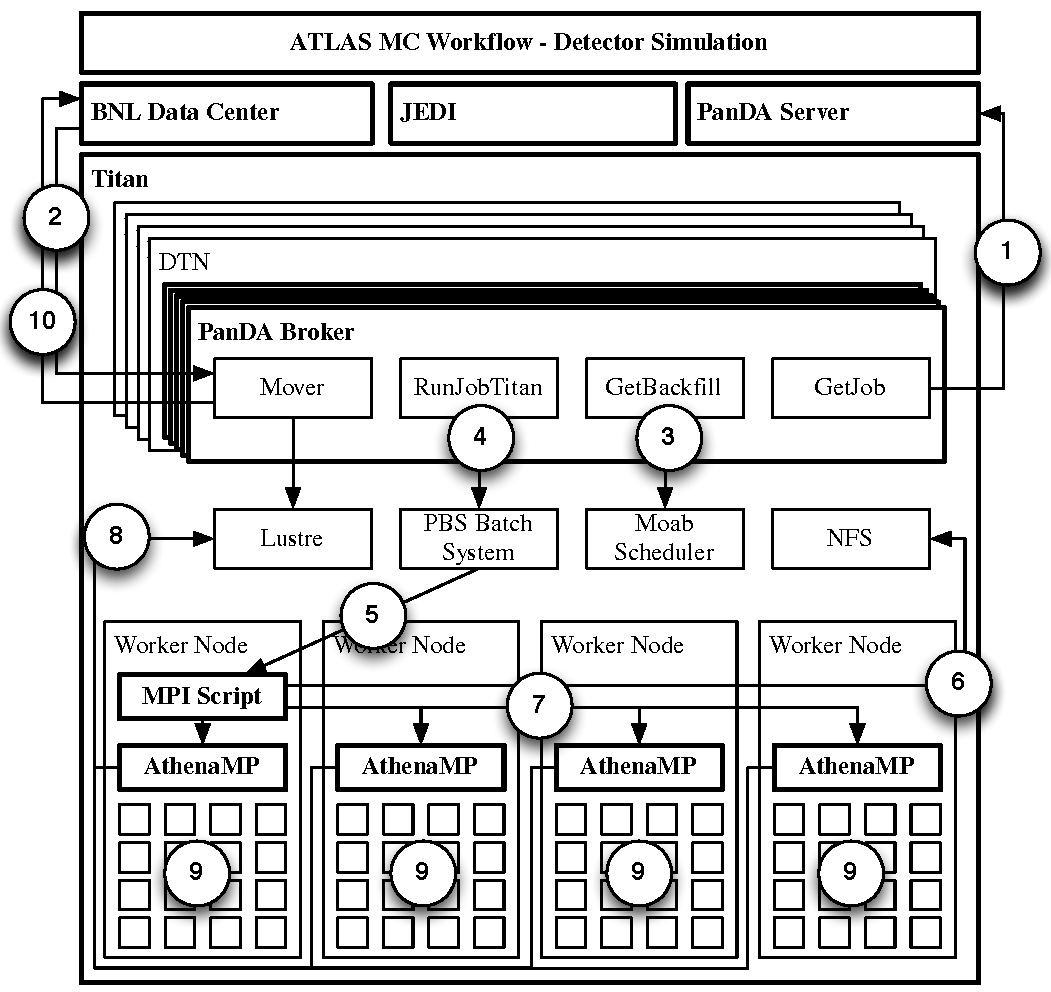
\includegraphics[width=\columnwidth]{panda_broker_architecture.pdf}
    \caption{PanDA Broker architecture as deployed on Titan. Numbers indicates
    the execution process of a detector simulation job, part of the production
    ATLAS MC workflow.}
\label{fig:panda_broker}
\end{figure}

Backfill querying is performed via a dedicated Moab scheduler command while a
tailored Python MPI script is used to execute the payload of ATLAS jobs. This
MPI script enables the execution of unmodified Grid-centric, ATLAS jobs on
Titan. Typically, a MPI script is workload-specific as it sets up the execution
environment for a specific payload. This involves organization of worker
directories, data management, optional input parameters modification, and
cleanup on exit. Upon submission, a copy of the MPI script runs on every
available worker node, starting the execution of the ATLAS job's payload in a
subprocess and waits until its completion.

MPI scripts are submitted to Titan's PBS batch system via
RADICAL-SAGA~\cite{radical-saga_url}, a Python module, compliant with the OGF
GFD.90 SAGA specification~\cite{goodale2008simple}. The Simple API for Grid
Applications (SAGA) offers a unified interface to diverse job schedulers and
file transferring services. In this way, SAGA provides an interoperability layer
that lowers the complexity of using distributed infrastructures. Behind the API
façade, RADICAL-SAGA implements a adaptor architecture: each adaptor interface
the SAGA API with different middleware systems and services, including the PBS
batch scheduler of Titan.

The data staging capabilities of the PanDA Broker are implemented via a file
system that is shared among DTNs and worker nodes. The input files with the
events of the ATLAS jobs are downloaded on the shared filesystem from the data
center of Brookhaven National Laboratory (BNL). The MPI script setup process
includes making the location of these files available to the payload of the
ATLAS's jobs. The PanDA Broker can locate the payload's output files on the
shared filesystem and transfer them from Titan BNL.

Once deployed on Titan, every PanDA Broker supports the execution of MC detector
simulations in 9 steps. PanDA Broker queries the Job Dispatcher module of the
PanDA server for ATLAS jobs that have been bound to Titan by JEDI
(Fig.~\ref{fig:panda_broker}:1). Upon receiving jobs descriptions, PanDA Broker
pulls jobs' input files from BNL to the OLCF Lustre file system
(Fig.~\ref{fig:panda_broker}:2). PanDA Broker queries Titan's Moab scheduler
about the current available backfill slot (Fig.~\ref{fig:panda_broker}:3) and
creates an MPI script, wrapping enough ATLAS jobs' payload to fit the backfill
slot. PanDA Broker submits the MPI script to the Titan's Torque batch system via
RADICAL-SAGA (Fig.~\ref{fig:panda_broker}:4).

Upon execution on the worker node(s) (Fig.~\ref{fig:panda_broker}:5), the MPI
script initializes and configures the execution environment
(Fig.~\ref{fig:panda_broker}:6), and executes one AthenaMP for each available
work node (Fig.~\ref{fig:panda_broker}:7). AthenaMP retrieves events from Lustre
(Fig.~\ref{fig:panda_broker}:8) and spawns 1 Geant4 event simulation process on
each of the 16 available cores (Fig.~\ref{fig:panda_broker}:9). Upon completion
of each MPI script, PanDA Broker transfer the jobs' output to BNL
(Fig.~\ref{fig:panda_broker}:10), and performs cleanup.

While PanDA Broker implementation is resource specific, it was successfully
ported to other supercomputers, including the HPC2 at the National Research
Center ``Kurchatov Institute'' (NRC-KI)~\cite{belyaev2015integration},
Edison/Cori at the National Energy Research Scientific Computing Center
(NERSC)~\cite{barreiro2016panda}, and SuperMUC at the Leibniz Supercomputing
Centre (LRZ)~\cite{barreiro2016panda}.


% ----------------------------------------------------------------------------
% IV - ANALYSIS AND DISCUSSION
% ----------------------------------------------------------------------------
\section{Analysis and Discussion}
\label{sec:panda_titan}

Currently, ATLAS deploys 20 instances of the PanDA Broker on 4 Titan's DTNs, 5
instances per DTN. Each broker submits and manages the execution of 15 to 300
ATLAS jobs, one job for each Titan's worker node, and a theoretical maximum
concurrent use of 96,000 cores. Since November 2015, PanDA Brokers have operated
only in backfill mode, without a defined time allocation, and running at the
lowest priority on Titan.

We evaluate the efficiency, scalability and reliability of the deployment of
PanDA WMS on Titan by characterizing the behavior of both PanDA Broker and
AthenaMP. We discuss challenges and limitations of our approach at multiple
levels arising from the specifics of workload, middleware and methods. All the
measurements were performed between January 2016 and February 2017, hereafter
called ‘experiment time window

% -----------------------------------------------------------------------------
\subsection{Characterizing the PanDA Broker on Titan}
\label{ssec:broker_titan}

We calculate the total amount of backfill availability over a period of time by:
(i) polling the available backfill slots at regular intervals during that time
window; (ii) converting the number of worker nodes available and their walltime
into core-hours; (iii) summing the number of core-hours. We call this number of
core-hours `total backfill availability'.

Fig.~\ref{fig:backfill-utilization} shows the total backfill availability on
Titan (gray bars) and the number of core-hours of that availability used by
ATLAS (blue bars) during the experiment time window. ATLAS consumed a total of
51.4M core-hours, for an average of $\approx$3.7M core-hours a month, with a
minimum of 1.7M core-hours in April 2016 and a maximum 7.9M core-hours in
February 2017.

\begin{figure}[!t]
    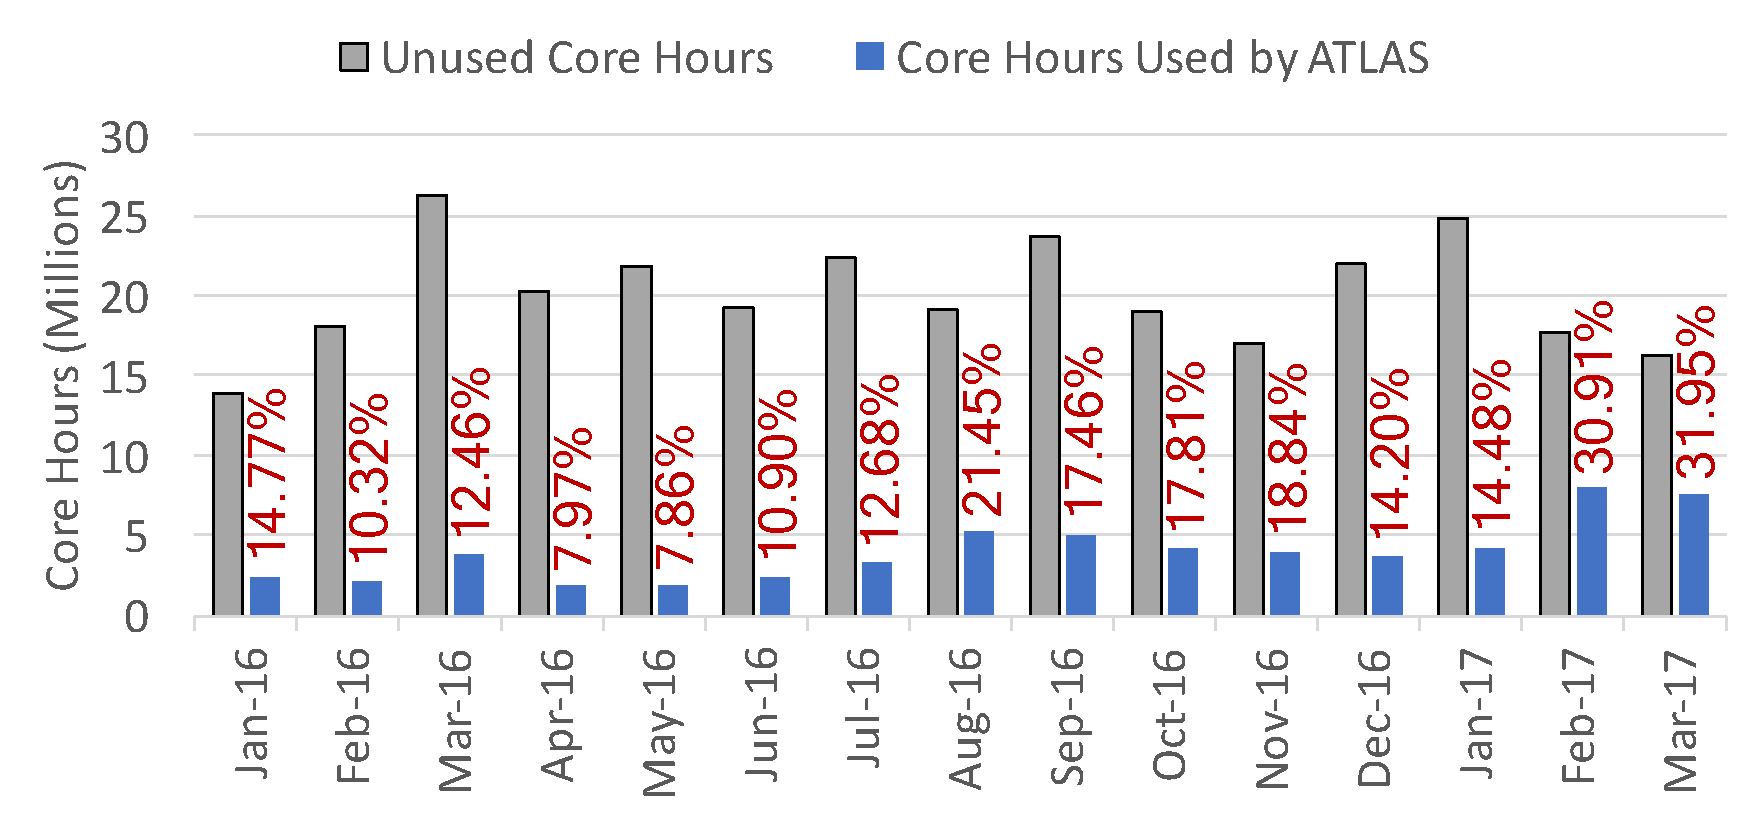
\includegraphics[clip,width=\columnwidth]{backfill_consumption.pdf}
    \caption{Titan's total backfill availability: CPU core-hours (gray) and CPU
    core-hours used by ATLAS (blue). GPU core-hours unaccounted for as they
    cannot be used by ATLAS. Efficiency of PanDA Brokers defined as percentage
    of total Titan's backfill availability used by ATLAS (Red labels).}
\label{fig:backfill-utilization}
\end{figure}

PanDA Brokers' efficiency (Fig.~\ref{fig:backfill-utilization}, red labels) is
defined as the fraction of core-hours utilized by the PanDA Brokers to  Titan’s
total backfill availability during the experiment time window. The brokers
reached 18\% average efficiency, with a minimum 7.8\% efficiency on May 2016 and
a maximum 30.9\% efficiency on February 2017 (excluding the preliminary results
of March). The total backfill availability was 20.3M in April 2016, and 17.6M in
February 2017. This shows that the measured difference in efficiency did not
depend on a comparable difference in the total backfill availability.

During the experiment time window, about 2.25M detector simulation jobs were
completed on Titan, for a total of 225M events processed. This is equivalent to
0.9\% of all the 250M detector simulations performed by ATLAS in the same period
of time, and 3.5\% of the 6.6B events processed by those jobs. These figures
confirms the relevance of supercomputers' resource contribution to the LHC Run
2, especially when accounting for the amount of unused total backfill
availability and the improvement of PanDA efficiency across the experiment time
window.

On February 2017, PanDA Brokers used almost twice as much total backfill
availability than in any other month (preliminary results for March 2017
displayed in Fig.~\ref{fig:backfill-utilization} confirm this trend). No
relevant code update was made during that period and logs indicated that the
brokers were able to perform faster. This is likely due to hardware upgrades on
the DTNs. The absence of continuous monitoring of those nodes does not allow to
quantify bottlenecks but spot measurements of their load indicate that a faster
CPU and better networking were likely responsible for the improved performance.
Investigations showed an average CPU load of 3.6\% on the upgraded DTNs. As
such, further hardware upgrades seem unlikely to improve significantly the
performance of PanDA Brokers.

Every detector simulation executed on Titan process 100 events. This number of
events is consistent with the physics of the use case and with the average
duration of backfill availability. The duration of a detector simulation is a
function of the number of events simulated but not all events take the same time
to be simulated. 1 event simulation takes from $\approx$2 to $\approx$40
minutes, with a mean of $\approx$14 minutes. Considering that each worker node
process up to 16 events concurrently, 100 events takes an average of 105 minutes
to process. As such, PanDA brokers do not use backfill availability with less
than 105 minutes walltime.

Fig.~\ref{fig:backfill-distrib} shows the distribution of backfill availability
on Titan as a function of number of nodes and the time of their availability
(i.e., walltime). We recorded these data by polling Titan's Moab scheduler at
regular intervals during the experiment window time. The mean number of nodes
was 691, and their mean walltime was 126 minutes. Detector simulations of 100
events, enable to use down to 5/6 of the mean walltime of backfill availability.
As such, it offers a good compromise for PanDA Broker efficiency.

\begin{figure*}[!t]
    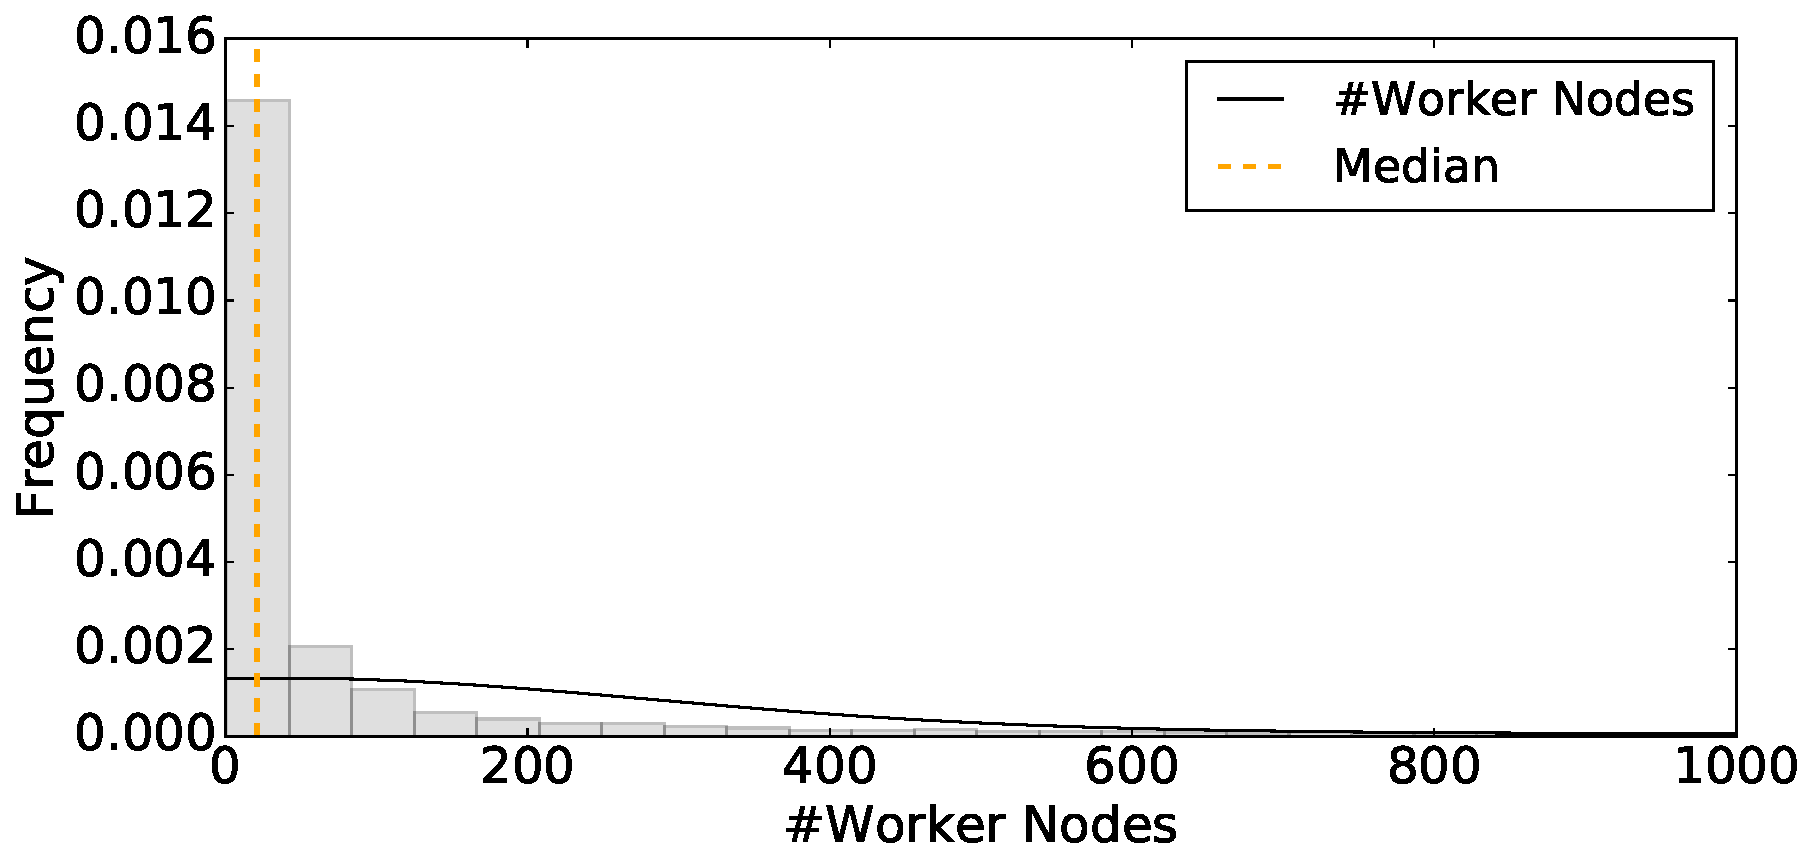
\includegraphics[clip,width=0.32\textwidth]{titan_backfill_wnodes_distribution.pdf}
    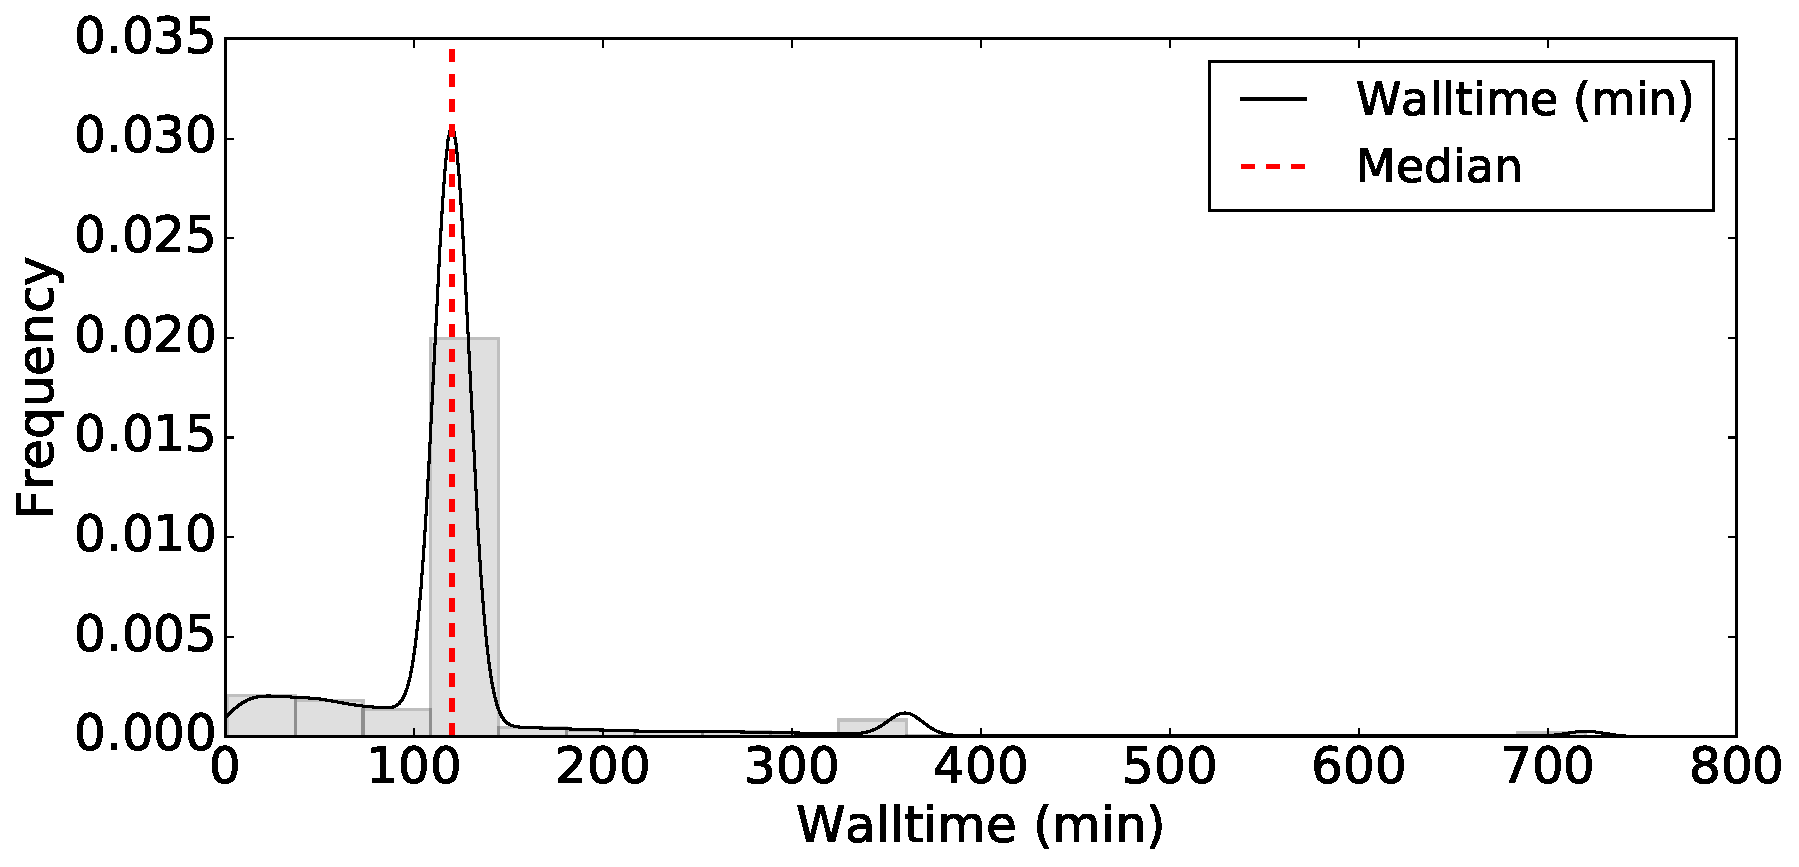
\includegraphics[clip,width=0.32\textwidth]{titan_backfill_walltime_distribution.pdf}
    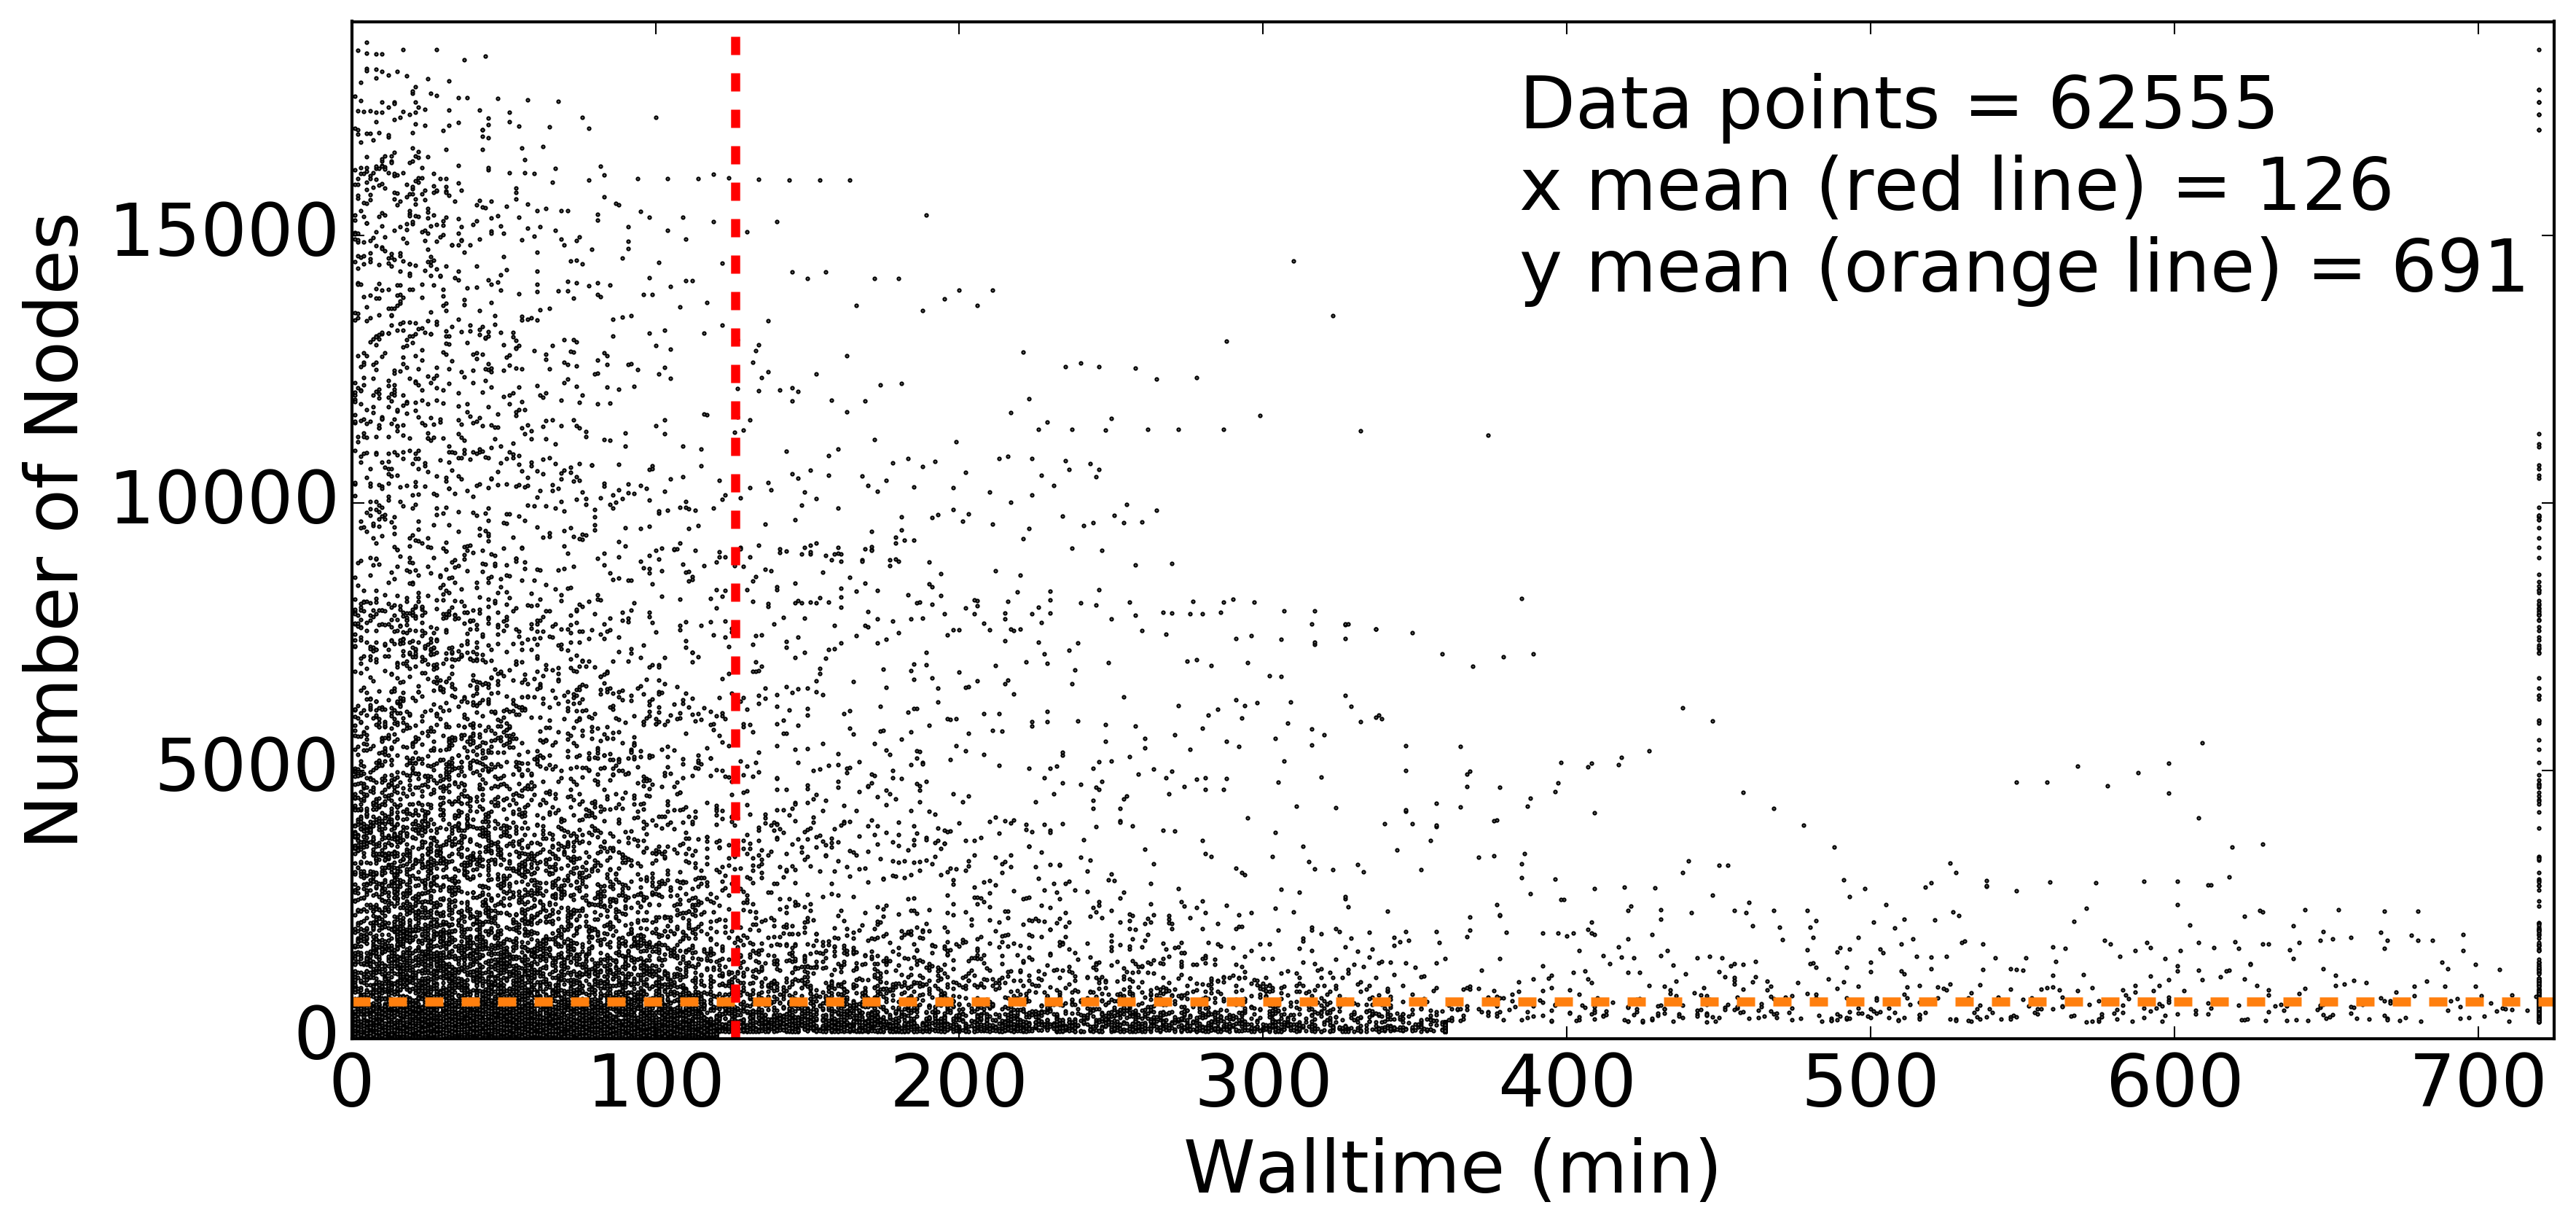
\includegraphics[clip,width=0.32\textwidth]{titan_backfill_avail.png}
    \caption{Backfill availability: distribution of number of work nodes (left)
    and of walltime in minutes (center). Scatter plot of the two variables
    (right). 62175 measures: mean number of work nodes available 691; mean
    walltime available 126 minutes.}
\label{fig:backfill-distrib}
\end{figure*}

PanDA Broker could fit the number of events to the walltime of each available
backfill slot on the base of the distributions of the time taken by one event to
be simulated. That specific number of event could then be pulled from the PanDA
Event service~\cite{calafiura2015atlas} and given as input to one or more
simulations. Once packaged into the MPI script submitted to titan's PBS batch
system, these simulations would better fit their available backfill slot,
contributing to increase the efficiency of PanDA Brokers.

The transition from a homogeneous to a heterogeneous number of events per
detector simulation has implications for the application layer. An even number
of events across simulations makes it easier to partition, track and package
events across simulations, especially when they are performed on both the Grid
and Titan. A homogeneous number of events also helps to keep the size and
duration of other stages of the MC workflow (\S\ref{ssec:panda-titan}) more
uniform. Further analysis is needed to evaluate the trade offs between increased
efficiency of resource utilization and the complexity that would be introduced
at the application layer.

Currently, each PanDA Broker creates, submits, and monitors a single MPI PBS
script at a time. This design is inherited from PanDA Pilot where a single
process is spawn at a time to execute the payload. As a consequence, the
utilization of a larger portion of Titan's total backfill availability depends
on the the number of concurrent PanDA Brokers instantiated on the DTNs: When all
the 20 PanDA Brokers have submitted a MPI PBS script, further backfill
availability cannot be used.

In September 2016, increasing the number of concurrent PanDA brokers from 4 to
20 markedly improved efficiency (see Fig.~\ref{fig:backfill-utilization}) but
further research is undergoing to understand whether an even larger number of
brokers would yield similar results. This research focuses on evaluating the
overheads of input/output files staging, including its impact on DTNs, and on an
alternative design of PanDA Broker that enables the concurrent submission of
multiple MPI scripts~\cite{barreiro2016panda}.

The current design and architecture of the PanDA Broker is proving to be as
reliable as PanDA Pilot when used on the WLCG. Between Jan 2016 and Feb 2017,
the overall failure rate of all the ATLAS detector simulation jobs was 14\%,
while the failure rate of jobs submitted to Titan was a comparable 13.6\%. PanDA
Brokers were responsible for around the 19\% of the failures, compared to the
29\% of failures produced by the JobDispatcher module of the PanDA Server, and
the 13\% failures produced by the Geant4 toolkit. The current failure rate of
the PanDA Brokers confirms the benefits of reusing most of the code base of the
PanDA Pilot for implementing the PanDA Broker. It also shows that adopting
third-party libraries like RADICAL-SAGA did not have a measurable adverse effect
on reliability.


% -----------------------------------------------------------------------------
\subsection{Characterizing the Detector Simulation on Titan}
\label{ssec:athenamp_titan}

We use two main parameters to measure the performance of the detector simulation
jobs submitted to Titan: (i) the time taken to setup AthenaMP; and (ii) the
distribution of the time taken by the Geant4 toolkit to simulate a certain
number of events.

AthenaMP has an initialization and configuration stage. At initialization time,
AthenaMP is assembled from a large number of shared libraries, depending on the
type of payload that will have to be computed. Once initialized, every algorithm
and service of AthenaMP is configured by a set of Python scripts. Both these
operations result in a large number of read operations on the filesystem shared
between the worker nodes and the DTNs, including the operations required to
access small python scripts.

Initially, all the shared libraries of AthenaMP and the python scripts for its
configuration were stored on the Spider 2 Lustre file system. However, the I/O
patterns of the initialization and configuration stages degraded the performance
of the filesystem. This was addressed by moving the AthenaMP distribution to a
read-only NFS directory, shared among DTNs and worker nodes. NFS eliminated the
problem of metadata contention, improving metadata read performance from
$\approx$6,300 seconds on Lustre to $\approx$1,500 seconds on NFS.

Once initialized and configured, AthenaMP is used to execute 16 concurrent
Geant4 simulators on a Titan's worker node. Geant4 requires to read events
descriptions from a filesystem and simulate them as they would happen within the
ATLAS detector. We characterized both the compute performance of the simulation
and the impact of acquiring event descriptions on the filesystem.

The AMD Opteron 6274 CPU used on Titan has 16 cores, divided into 8 compute
units. Each compute units has 1 floating point (FP) scheduler shared between 2
cores. When using 16 cores for FP-intensive calculations, each pair of cores
competes for a single FP scheduler. This creates the overhead shown in
Fig.~\ref{fig:comparison-8-16cores}: the mean runtime per event for 8
concurrent simulations computing 50 events is 10.8 minutes, while for 16
simulations is 14.25 minutes (consistent with the measured distribution of the
duration of event simulation). Despite an inefficiency of almost 30\%, Titan's
allocation policy based on number of worker nodes used instead of number of
cores does not justify the use of 1/2 of the cores available.

\begin{figure}[htp]
    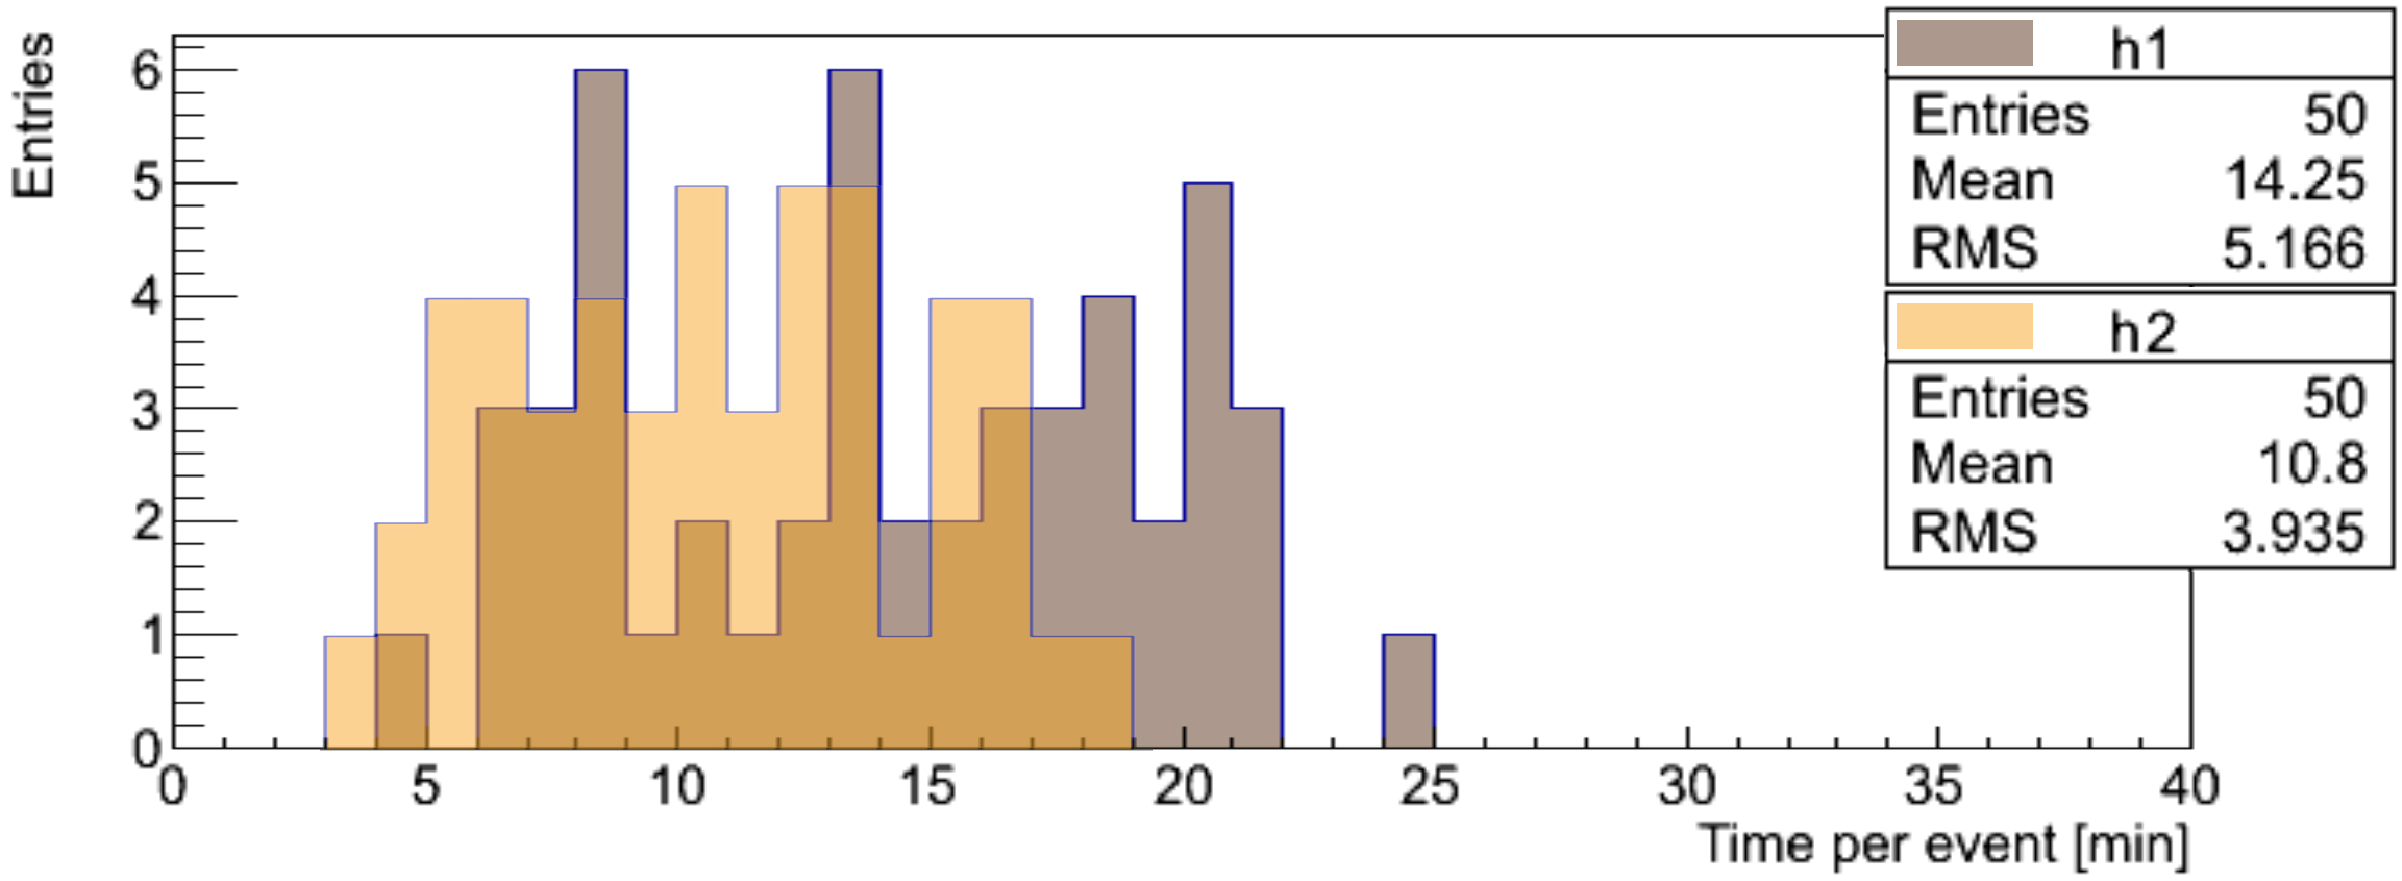
\includegraphics[clip,width=\columnwidth]{tx8_tx16_comparison_vsquashed.pdf}
    \caption{Distributions of the time taken to simulate one event when placing
    2 simulations (h1) or 1 simulation (h2) per Titan's CPU. 2 simulation use 16
    cores per node, 1 simulation 8. 50 Events; 1 Titan worker nodes; 16 work
    threads per node; 100 events per node.}
\label{fig:comparison-8-16cores}
\end{figure}

The performance analysis of Titan's AMD CPUs for detector simulations helps also
to compare Titan and Grid site performances. Usually, Grid sites exposes
resources with heterogeneous CPU architectures and a maximum of 8 (virtual)
cores per worker node, while Titan's offer an homogeneous 16 cores architecture.
We used the rate of events processes per minute as a measure of the efficiency
of executing the same detector simulation on Titan or Grid sites. Comparisons of
the efficiencies of Titan to the BNL and SIGNET Grid sites, normalized for 8
cores, show that the effective performance per-core at Titan is $\approx$0.57
event per minute, roughly 1/2 of BNL and  1/3 of SIGNET performances.

The differences in performance between Titan and the BNL and SIGNET Grid sites
are due to the FP scheduler competition and the availability of newer
processors. The CPUs at the Grid sites have one FP scheduler per core and are on
average newer than the CPU of Titan. The heterogeneity of the Grid sites' CPUs
explain the higher performance variance we observed compared to the performance
consistency we measured on Titan.

We studied the impact of acquiring event descriptions on Lustre by analyzing
1,175 jobs ran on the week of 10/25/2016, for a total of 174 hours.
Table~\ref{panda-olcf-stats} shows the overall statistical breakdown of the
observed file I/O. ATLAS used between 1 and 300 worker nodes, and 35 on average.
75\% of the jobs run by ATLAS consumed less than 25 nodes and 92\% less than
100. During the 174 hours of data collection, 6.75 ATLAS jobs were executed on
average per hour, each job running for an average of 1.74 hours. Every job read
less than 250 GB and wrote less than 75 GB of data and, on average, each job
read 20 GB and wrote 6 GB of data.

\begin{table*}[t]
\centering
\begin{tabular}{lllllllll}
 & Num. Nodes & Duration (s) & Read (GB) & Written (GB) & GB Read/nodes & GB Written/nodes & $open()$ & $close()$ \\
Min & 1 & 1,932 & 0.01 & 0.03 & 0.00037 & 0.02485 & 1,368 & 349 \\
Max & 300 & 7,452 & 241.06 & 71.71 & 0.81670 & 0.23903 & 1,260,185 & 294,908 \\
Average & 35.66 & 6,280.82 & 20.36 & 6.87 & 0.38354 & 0.16794 & 146,459.37 & 34,155.74 \\
Std. Dev. & 55.33 & 520.99 & 43.90 & 12.33 & 0.19379 & 0.03376 & 231,346.55 & 53,799.08
\end{tabular}
\caption{The Statistical breakdown of the I/O impact of 1,175 jobs ATLAS executed at OLCF for the week of 10/25/16}
\label{panda-olcf-stats}
\end{table*}

ATLAS jobs are read heavy: On average, the amount of data read per worker node
is less than 400 MB, while the amount of data written is less than 170 MB.
Distributions of read and written data are different: The read operation
distribution per job shows a long tail, ranging from 12.5 GB to 250 GB, while
the written amount of data has a very narrow distribution.

The metadata I/O breakdown shows that ATLAS jobs yield 23 file $open()$
operations per second (not including file $stat()$ operations) and 5 file
$close()$ operations per second, with similar distributions. On average, the
maximum number of file $open()$ operations per job is $\approx$170/s and the
maximum number of file $close()$ operations is $\approx$39/s. For the 1,175
ATLAS jobs observed, the total number of file $open()$ operations is 172,089,760
and the total number of file $close()$ operations is 40,132,992. The difference
between these two values is still under investigation: One possible explanation
is that ATLAS jobs don't call a file $close()$ operation per every file $open()$
issued.

Overall, the average time taken to read events from input files stored on Lustre
is 1,320, comparable to the time taken to read the file required by assembling
AthenaMP from NFS. Preliminary investigation shows that this time could be
reduced to 40 seconds by loading the event descriptions into the RAM disk
available on each worker node. Events descriptions could be transferred from
Lustre to the RAM disk while configuring and initializing AthenaMP, almost
halving the time currently required by initiating a Genat4 simulation.



% ----------------------------------------------------------------------------
% VI - THE NEXT GENERATION EXECUTOR
% ----------------------------------------------------------------------------
% \section{PANDA: Future/RoadMap}
\section{PANDA\@: The Next Generation Executor}
\label{sec:panda_roadmap}

As seen in \S\ref{ssec:panda_titan}, PanDA Broker was  deployed on the DTNs
as Titan's worker nodes lack connectivity to the wide area network The lack of
pilot capabilities impacts both the efficiency and the flexibility of PanDA's
execution process. Pilots could improve efficiency by increasing throughput and
enabling greater backfill utilization. Further, pilots makes it easier to
support heterogeneous workloads.

The absence of pilots imposes the static coupling between MPI scripts
submitted to the PBS batch system and detector simulations
(\S\ref{sec:panda_titan}). This makes the scheduling of multiple generations
of workload on the same PBS job impossible: once a statically defined number
of detector simulations are packaged into a PBS job and this job is queued on
Titan, no further simulations can be added to that job. New simulations have
to be packaged into a new PBS job that needs to be submitted to Titan based
upon backfill availability.

The support of  multiple generations of workload would enable more efficient use
of the backfill availability of walltime. Currently, when a set of simulations
ends, the PBS job also ends, independent of whether more wall-time would still
be available. With a pilot, additional simulations could be executed  to utilize
all the available wall-time, while avoiding further job packaging and submission
overheads.

Multiple generations would also relax two assumptions of the current execution
model: knowing the number of simulations before submitting the MPI script, and
having a fixed number of events per simulation (100 at the moment). Pilots would
enable the scheduling of simulations independently from whether they were
available at the moment of submitting the pilot. Further, simulations with a
varying number of events could be scheduled on a pilot, depending on the amount
of remaining walltime and the distribution of execution time per event, as shown
in \S\ref{ssec:panda_titan}, Fig.~\ref{fig:comparison-8-16cores}. These
capabilities would increase the efficiency of the PanDA Broker when there is a
large difference between the number of cores and walltime.

Pilots can offer a payload-independent scheduling interface while hiding the
mechanics of coordination and communication among multiple worker nodes. This
could eliminate the need for packaging payload into MPI scripts within the
broker, greatly simplifying the submission process. This simplification would
also enable the submission of different types of payload, without having to
develop a specific PBS script for each payload. The submission process would
also be MPI-independent, as MPI is used for coordination among multiple worker
nodes, not by the payload.

% -----------------------------------------------------------------------------
\subsection{Implementation}
\label{sec:arch}

The implementation of pilot capabilities within the current PanDA Broker require
quantification of the effective benefits that it could yield and, on the base of
this analysis, a dedicated engineering effort. We developed a prototype of a
pilot system capable of executing on Titan to study experimentally the
quantitative and qualitative benefits that it could bring to PanDA. We called
this prototype Next Generation Executor (NGE).

NGE is a runtime system to execute heterogeneous and dynamically determined
tasks that constitute workloads. Fig.~\ref{fig:arch-overview} illustrates its
current architecture as deployed on Titan: the two management modules (Pilot
and Unit) represent a simplified version of the PanDA Broker while the agent
module is the pilot submitted to Titan and executed on its worker nodes. The
communication between PanDA Broker and Server is abstracted away as it
is not immediately useful to evaluate the performance and capabilities of a
pilot on Titan.

\begin{figure}
  \centering
   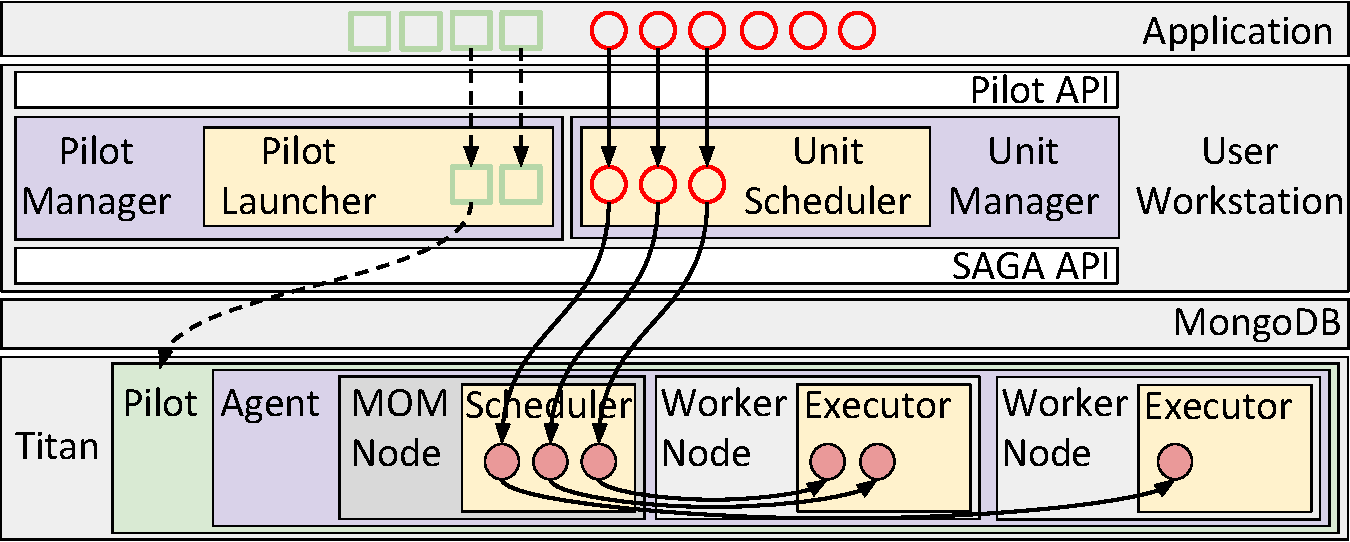
\includegraphics[width=\columnwidth]{rp_architecture_compact_atlaswms_paper.pdf}
  \caption{NGE Architecture: The PilotManager and  UnitManager reside on a Titan
  DTN while the Agent is executed on its worker nodes. Color coding: gray for
  entities external to NGE, white for APIs, purple for NGE's modules, green for
  pilots, yellow for module's components.}
\label{fig:arch-overview}
\end{figure}

NGE exposes an API to describe workloads (Fig.~\ref{fig:arch-overview}, green
squares) and pilots (Fig.~\ref{fig:arch-overview}, red circles), and to
instantiate a PilotManager and a UnitManager.   The PilotManager submits
pilots to Titan's PBS  batch system via SAGA API (Fig.~\ref{fig:arch-overview}, dash arrow), as done by PanDA Broker to submit MPI scripts. Once
scheduled, the pilot's Agent is bootstrapped on Titan's MOM node and
the Agent's Executors on the on the worker
nodes, and the UnitManager schedules units to the Agent's Scheduler
(Fig.~\ref{fig:arch-overview}, solid arrow). The Agent's Scheduler schedules
the units on one or more Agent's Executor for execution. The Agent's executors
can manage one or more worker nodes, depending on performance evaluations. The
UnitManager and the Agent communicate via a database that is instantiated on
one of Titan's DTN so as to be reachable by both modules.

The NGE Agent uses the \emph{Open Run-Time Environment (ORTE)} for
communication and coordination of the execution of units. This environment is
a critical component of the OpenMPI implementation, developed to support
distributed high-performance computing applications operating in a
heterogeneous environment~\cite{castain05:_open_rte, cug-2016}. ORTE provides
a mechanism to create a \emph{``dynamic virtual machine''} (DVM) that spans
multiple nodes. The DVM transparently provides support for interprocess
communication, resource discovery and allocation, and process launching across
a variety of platforms. Libraries enable the interaction between users and
ORTE to enable the submission, monitoring and managing of tasks, avoiding
filesystem bottlenecks and race conditions with network sockets. As a
consequence, ORTE is able to minimize the system overhead while submitting
tasks.

\subsection{Experiments}
\label{sec:ngeExp}

We designed experiments to characterize the performance of the NGE on Titan,
with an emphasis on understanding its overhead and thus the cost of introducing
new functionalities.  We perform three groups of experiments in which we
investigate the weak scalability, weak scalability with multiple generation, and
strong scalability of the NGE.

Each experiment entails executing multiple instances of AthenaMP
to simulate a pre-determined number of events. All the experiments have been
performed by  configuring AthenaMP to use all the 16 cores  of Titan's worker
nodes.

We  measured the execution time of the pilots and of AthenaMP
within them, collecting timestamps at  all stages of the execution. Experiments
were performed  by  submitting NGE's pilots  to Titan's batch queue.  The
turnaround time of an individual run is determined by queue waiting times. Since
we are interested only in the performances of the NGE, we removed queue time
from our statistics.

\subsubsection{Weak scalability}

In this experiment  we run as many AthenaMP instances (hereafter referred to as
tasks)  as the number of nodes controlled by the pilot. Each AthenaMP simulates
100 events, requiring $\sim 4200$ seconds on average.

Tasks do not  wait within the NGE Agent's queue since  one node  is available to
each AthenaMP instance.  Overheads in task execution are consequence primarily
of the three other factors: (i) the  initial bootstrapping of the pilot on the
nodes; (ii) the UnitManager's dispatching of  units (tasks) to the agent; and
(iii) time for the agent to bootstrap all the tasks on the nodes.

We tested  pilots  with 250, 500, 1000 and 2000 worker nodes and 2 hours
walltime. The time duration is determined by the Titan's walltime policy.
Fig.~\ref{fig:weakScal1a} depicts the average pilot duration, the average
execution time of AthenaMP, and the NGE pilot overhead as function of the pilot
size.

\begin{figure}[!t]
        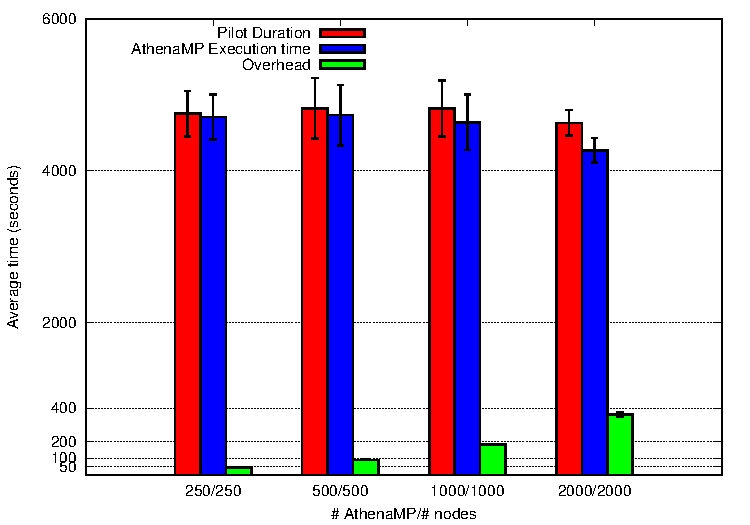
\includegraphics[height=4.5cm,width=\columnwidth]{weak1.pdf}
    \caption{Weak scalability: average pilot duration, average duration of one AthenaMP execution, and pilot's overhead as a function of pilot sizes (200, 500, 1000 and 2000 nodes).}
\label{fig:weakScal1a}
\end{figure}

We observe that, despite some fluctuations due to external factors (e.g.,
Titan's shared filesystem and the shared database used by the NGE), the average
execution time of AthenaMP  ranges between 4200 and 4800 seconds.  We  also
observe that in all the cases the gap between AthenaMP execution times and the
pilot durations is minimal, although it slightly increases with the pilot size.
We  notice that NGE's overhead does grow linearly with the number of units.

\subsubsection{Weak scalability with multiple generation }

The NGE provides an important new capability of submitting multiple generations
of AthenaMP to the same pilot. In order to investigate the cost of doing so, we
performed a variant of the weak scalability experiments. This stresses the
pilot's components, as new tasks are scheduled for execution on the Agent while
other tasks are still running.

In these experiments, we run five AthenaMP instances per node.  As these
experiments are designed to investigate the overhead generated by the scheduling
and bootstrap of AthenaMP instances, we reduced the number of events simulated
by each AthenaMP task to sixteen in such a way that the running time of each
AthenaMP is, on average, $\sim 1200$ seconds. This experiment design choice does
not affect the  objectives or accuracy of the experiments, but allows us to
scale experiments to large node counts by being conservative with allocation.

We ran pilots with 256, 512, 1024 and 2048 worker nodes and 3\mtnote{2?} hours
walltime. Fig.~\ref{fig:weakScal2a} depicts the average pilot duration, the
average execution time of five sequential generations of AthenaMP, and the
corresponding overhead. We observe that the difference between the two durations
is more marked than in the previous experiments. Despite this, we notice that
the growth of the overhead is consistent with the increment of the number of
tasks per node for pilots with 256, 512 and 1024 worker nodes, and less than
linear for the pilot with 2048 worker nodes.

\begin{figure}[!t]
        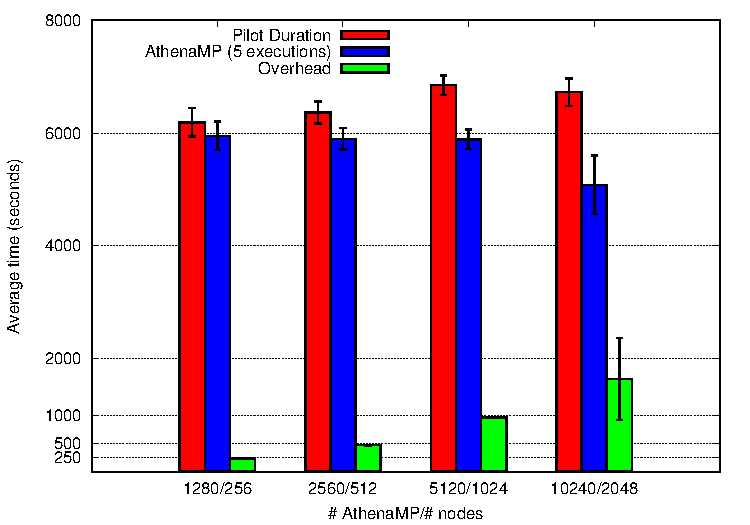
\includegraphics[height=4.5cm,width=\columnwidth]{weak2.pdf}
    \caption{Weak scalability with multiple generations: average pilot
    duration, average duration of sequential AthenaMP executions, and
    pilot's overhead for pilot with 256, 512, 1024 and 2048 nodes.}
\label{fig:weakScal2a}
\end{figure}

%\vspace{-0.2in}

\subsubsection{Strong scalability}

The last experiments  study strong scalability by running the same number of
tasks for different pilot sizes. We used 2048 AthenaMP instances and  pilots
with 256, 512, 1024 and 2048 nodes. Thus, the number of AthenaMP generations is
equal to eight times the size of the smallest pilot and corresponds to the size
of the largest pilot. As a consequence, the number of consecutive generations of
AthenaMP decreases with the pilot size by generating different dynamics within
the pilots. These experiments are designed to investigate whether pilot overhead
is affected by the degree of concurrency within the pilot and/or the number of
tasks. Each AthenaMP instance simulates sixteen events as in the previous
experiment.

Fig.~\ref{fig:strongScala}  shows the average pilot duration and the average
execution time of possibly sequential AthenaMP instances.  We  notice that the
difference between the pilot duration and the AthenaMP execution times is almost
constant for all the pilot sizes, although the overall duration of the pilot
decreases linearly with the pilot size.

\begin{figure}[!t]
        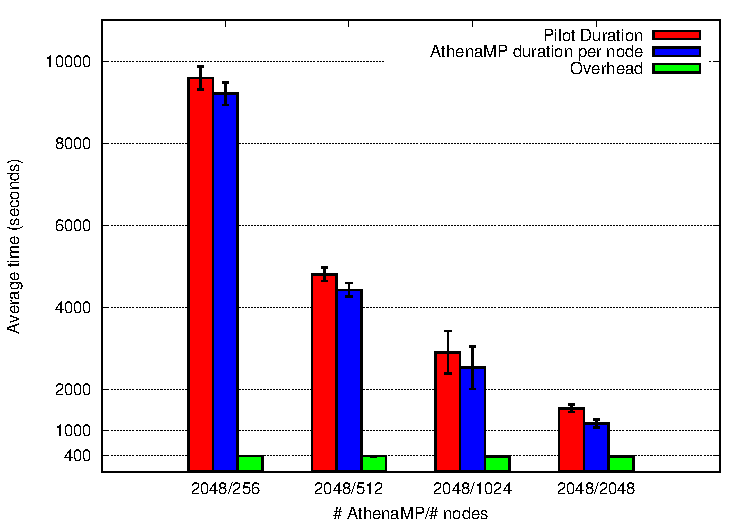
\includegraphics[height=4.5cm,width=\columnwidth]{strong.pdf}
    \caption{Strong scalability:  average pilot duration, average duration of
    sequential AthenaMP executions, and pilot's overhead for pilots with 256, 512, 1024 and 2048 nodes.}
\label{fig:strongScala}
\end{figure}


% ----------------------------------------------------------------------------
% VII - RELATED WORK
% ----------------------------------------------------------------------------
\section{Related Work}
\label{sec:related}

Several pilot-enabled WMS were developed for the LHC experiments:
AliEn~\cite{Bagnasco2010} for ALICE; DIRAC~\cite{Paterson2010} for LHCb;
GlideinWMS~\cite{sfiligoi2008glideinwms} for CMS; and
PanDA~\cite{maeno2014evolution} for ATLAS. These systems implement similar
design and architectural principles: centralization of task and resource
management, and of monitoring and accounting; distribution of task execution
across multiple sites; unification of the application interface; hiding of
resource heterogeneity; and collection of static and sometimes dynamic
information about resources.

AliEn, DIRAC, GlideinWMS and PanDA all share a similar design with two types of
components: the management ones facing the application layer and centralizing
the capabilities required to acquire tasks' descriptions and matching them to
resource capabilities; and resource components used to acquire compute and data
resources and information about their capabilities. Architecturally, the
management components include one or more queue and a scheduler that coordinates
with the resource modules via push/pull protocols. All resource components
include middleware-specific APIs to request for resources, and a pilot capable
of pulling tasks from the management modules and executing them on its
resources.

AliEn, DIRAC, GlideinWMS and PanDA also have similar implementations. These WMS
were initially implemented to use Grid resources, using one or more components
to the Condor software ecosystem~\cite{thain2005distributed} and, as with
GlideinWMS, contributing to its development. Accordingly, all LHC WMS
implemented Grid-like authentication and authorization systems and adopted a
computational model based on distributing a large amount of single/few-cores
tasks across hundreds of sites\mtnote{Is this true?}.

All the experiments at LHC produces and process large amount of data both from
actual collisions in the accelerator and from their simulations. Dedicated,
multi-tiered data systems have been built to store, replicate, and distributed
these data. All LHC WMS interface with these systems to move data to the sites
where related compute tasks are executed or to schedule compute tasks where
(large amount of) data are already stored.


% ----------------------------------------------------------------------------
% VIII - CONCLUSION
% ----------------------------------------------------------------------------
%\vspace{-0.1in}
\section{Conclusion}
\label{sec:conclusion}

The deployment of PanDA Broker on Titan enabled distributed computing on a
leadership-class HPC machine at unprecedented scale. In the past 13 months,
PanDA WMS has consumed almost 52M core-hours on Titan, simulating 3.5\% of the
total number of detector events of the ATLAS production Monte Carlo workflow. We
described the implementation and execution process of PanDA WMS
(\S\ref{sec:panda_overview}) and PanDA Broker (\S\ref{sec:panda_titan}), showing
how they support and enable distributed computing at this scale on Titan, a
leadership-class HPC machine managed by OCLF at ORNL.

We characterized the state of practice by evaluating the efficiency, scalability
and reliability of both PanDA Broker and AthenaMP as deployed on Titan
(\S\ref{sec:panda_titan}). Our characterization highlighted the strengths
and limitations of the current design and implementation: PanDA Brokers enable
the sustained execution of millions of simulations per week but further work is
required to optimize its efficiency and reliability (\S\ref{ssec:broker_titan}).
PanDA Brokers support the concurrent execution of multiple AthenaMP instances,
enabling each AthenaMP to perform the concurrent execution of up to 16 Geant4
simulators. Nonetheless, our characterization showed how improving I/O
performance could reduce overheads (\S\ref{ssec:athenamp_titan}), increasing the
overall utilization of Titan's backfill availability.

More generally, this paper highlights the fundamental role of WMS for
experimental science. HEP was amongst the first, if not the very first
experimental community to realize the importance of using WMS to manage their
computational campaign(s). As computing becomes increasingly critical for a
range of experiments, the impact of WMS on HEP foreshadows the importance of
WMS for other experiments (such as SKA, LSST etc.). % and their computational
campaigns. These experiments will have their own workload characteristics,
resources types and federation constraints, as well metrics of performance.
The design and experience captured in this paper will prove invaluable for
designing WMS to support computational campaigns and will provide a baseline
to evaluate the relative merits of different approaches.

The 52M core hours used by ATLAS, via PanDA, is over 2\% of the total
utilization on Titan over the same period, bringing the time-averaged
utilization of Titan to be consistently upwards of 90\%. Given that the
average average utilization of most other leadership class machines is less
(e.g., NSF's flagship Blue Waters the average utilization fluctuates between
60-80\% (see XDMoD\cite{bw-sucks})) there is ample headroom for similar
approaches elsewhere. These unprecedented efficiency gains aside, this work is
just a starting point towards more effective operational models for future
leadership and online analytical platforms~\cite{foap-url}. These platforms
will have to support ever increasing complex workloads with varying models for
dynamic resource federation. Recent efforts with Google Cloud for the CMS
experiment -- HEPCloud~\cite{hepcloud,googlehep} represent similar yet
different approaches to dynamic resource federation. As the type,
heterogeneity and complexity of future platforms  (e.g., Exascale, Commercial
Clouds) for science increases, there will be a greater need and emphasis on
abstractions to ensure WMS can both utilize as well as support evolving
platforms. Our experience demonstrated the advantages arising from an
abstractions based approach \textendash{} in particular scalable implementations
of pilot abstraction.


% ----------------------------------------------------------------------------
% ACKNOWLEDGEMENTS
% ----------------------------------------------------------------------------
\section*{Acknowledgements}
\label{sec:ack}

This research used resources of the Oak Ridge Leadership Computing Facility,
supported by the Office of Science of the Department of Energy under Contract
DE-AC05-00OR22725.

% ----------------------------------------------------------------------------
% REFERENCES
% ----------------------------------------------------------------------------
\bibliographystyle{IEEEtran}
\bibliography{bibliography}

% that's all folks
\end{document}
